\documentclass[12pt, a4paper, UTF8, openany]{ctexbook}

\usepackage{geometry}%设置页边距
\geometry{left=1.54cm, right=1.54cm, top=2.18cm, bottom=2.18cm}

\usepackage{tikz}%绘图
\usetikzlibrary{calc}%绘图时计算
\usetikzlibrary{angles}%角度标识
\usetikzlibrary{intersections}%计算交点

\usepackage{amsmath, amssymb}%数学
\usepackage{esint}%Extended set of integrals
\usepackage{extarrows}%Extended Arrows

\usepackage{array}%表格基础设置
\usepackage{longtable}%跨页表格
\usepackage{booktabs}%表格水平线

\usepackage{multicol}%多列

\usepackage[colorlinks = true, linkcolor = black]{hyperref}%超链接跳转

\usepackage{color}

\newcommand{\dif}{\mathrm{d}}
\newcommand{\Dif}{\mathrm{D}}
\newcommand{\difx}{\,\mathrm{d}x}
\newcommand{\dify}{\,\mathrm{d}y}
\newcommand{\sdif}{\,\dif}

\newcommand{\difk}[2]{{#1}^{(#2)}}

\newcommand{\field}[1]{\mathbb{#1}}%域

\newcommand{\imunit}{\mathrm{i}}%虚数单位

\newcommand{\poly}{\mathrm{Poly}}

\newcommand{\mat}[1]{\mathbf{#1}}

\newcommand{\R}[1]{\field{R}^{#1}}

\newcommand{\uzero}{\mathop{U}\limits^{\circ}}%空心邻域
\newcommand{\eps}{\varepsilon}

\newcommand{\len}[1]{||\, #1 \,||}%向量的模

\newcommand{\inter}[1]{\text{int }{#1}}%内部
\newcommand{\exter}[1]{\text{ext }{#1}}%外部
\newcommand{\border}[1]{\partial{#1}}%边界

\newcommand{\closure}[1]{\overline{#1}}

\newcommand{\grad}{\mathrm{grad}}
\newcommand{\divf}{\mathrm{div}}
\newcommand{\rot}{\mathrm{rot}}

\newcommand{\grads}{\mathrm{grad}\,}
\newcommand{\divfs}{\mathrm{div}\,}
\newcommand{\rots}{\mathrm{rot}\,}

\newcommand{\inner}[2]{\langle #1, #2 \rangle}

\newcommand{\colalign}[2]{\multicolumn{1}{#1}{#2}}%控制单格对齐方式

\linespread{1.05}%行间距
\setlength{\parskip}{8pt}%段落间距
\setlength{\parindent}{0pt}%不缩进

\setcounter{chapter}{-1}

\title{Analysis}
\author{1001}

\begin{document}
    \maketitle

    \tableofcontents
    \cleardoublepage

    \chapter{引言}
    \begin{longtable}[2]{*{2}{w{l}{9cm}}}
        $\csc x = 1 / \sin x$ & $\sec x = 1 / \cos x$ \\
        $\cot^2 x + 1 = \csc^2 x$ & $\tan^2 x + 1 = \sec^2 x$ \\
        & \\
        $\sin x + \sin y = 2 \sin \dfrac{x + y}{2} \cos \dfrac{x - y}{2}$ & 
        $\sin x \cos y = \dfrac{1}{2}\left(\sin(x + y) + \sin(x - y)\right)$ \\
        \addlinespace
        $\sin x - \sin y = 2 \cos \dfrac{x + y}{2} \sin \dfrac{x - y}{2}$ & 
        $\cos x \sin y = \dfrac{1}{2}\left(\sin(x + y) - \sin(x - y)\right)$ \\
        \addlinespace
        $\cos x + \cos y = 2 \cos \dfrac{x + y}{2} \cos \dfrac{x - y}{2}$ &
        $\cos x \cos y = \dfrac{1}{2}\left(\cos(x + y) + \cos(x - y)\right)$ \\
        \addlinespace
        $\cos x - \cos y = {\color{red}-}2 \sin \dfrac{x + y}{2} \sin \dfrac{x - y}{2}$ &
        $\sin x \sin y = {\color{red}-}\dfrac{1}{2}\left(\cos(x + y) - \cos(x - y)\right)$
    \end{longtable}

    \chapter{函数，极限，连续}

    \section{基础}
    有界；有上/下确界 $\sup / \inf$。

    {\heiti 完备性}：有上/下界的非空实数集有上/下确界。

    单调：含等号。严格单调。

    邻域：$U(x_0, \eps) := \{x : |x - x_0| < \eps\}$。\\
    去心邻域：$\uzero(x_0, \eps) := U(x_0, \eps) \backslash \{x_0\}$。
    
    \section{极限}
        \subsection{定义}
        数列极限：$\forall \eps > 0$，$\exists N \in \field{N}_+$，使得 $\forall n > N$，$|a_n - A| < \eps$。

        函数极限：趋于无穷类似\\
        （Cauchy）$\eps-\delta$ 式：
        $\forall \eps > 0$，$\exists \delta > 0$，使得 $\forall x \in \uzero(x_0, \delta)$，$|f(x) - A| < \eps$。\\
        （Heine）序列式：$\forall x_n \to x_0$，$\lim_{n \to \infty} f(x_n) = A$。

        左极限 $x \to x_0^-$，右极限 $x \to x_0^+$。\\
        $\lim_{x \to x_0} = A \iff \lim_{x \to x_0^{-}} = \lim_{x \to x_0^{+}} = A$。

        \subsection{性质}
        极限唯一。\\
        证明：反证。取 $\eps = \frac{A + B}{2}$，即得矛盾。

        有界性：数列有界，函数局部有界。（上下均有界。）

        保序性：$\forall l_n \leqslant a_n \leqslant r_n$，则 $\lim l \leqslant \lim a \leqslant \lim r$。\\
        函数局部保序。\\
        推论：保号性。局部保号性。

        收敛数列的任意子列均收敛于 $A$。\\
        函数版本即 Heine 定理（序列式定义）。

        四则运算，函数复合。{\heiti 前提}：有定义。

        \subsection{判别与求值}
        单调有界准则。

        夹逼准则。

        归并原理：研究子列极限。数列、函数均可\\
        {\heiti 应用}：证明发散。

        闭区间套：$\{[a_n, b_n]\}$，满足 $[a_1, b_1] \supset [a_2, b_2] \supset \cdots$，且长度趋于零 $\lim b_n - a_n = 0$。\\
        闭区间套原理：存在{\heiti 唯一} $\xi$，使得 $\cap [a_i, b_i] = \{\xi\}$。证明：夹逼。

        Weierstrass 定理：有界数列必有收敛子列。\\
        证明：每次对分值域区间，总有一个子区间含有无穷多项。在另一子区间任取 $x_n$，在无穷多的子区间内递归。
        值域区间构成闭区间套，则构造了收敛子列 $\{x_n\}$。\\
        {\heiti 应用}：先构造极限值 $A$，再证明收敛于 $A$。

        Cauchy 数列 $\{a_n\}$：满足 $\forall \eps > 0$，$\exists N \in \field{N}_+$，
        使得 $\forall m, n > N$，$|a_m - a_n| < \eps$。\\
        等价叙述：$\forall n > N, p \in \field{N}_+$，$|a_n - a_{n + p}| < \eps$。

        Cauchy 收敛原理：\\
        a. $\{a_n\}$ 收敛的充要条件是 $\{a_n\}$ 为 Cauchy 列。证明：取 $\eps / 2$。\\
        b. $\lim_{x \to x_0} f(x)$ 存在的充要条件是 $\forall \eps > 0$，$\exists \delta > 0$，
        使得 $\forall x_1, x_2 \in \uzero(x_0, \delta)$，$|f(x_1) - f(x_2)| < \eps$。
        证明：充分性同数列；必要性需证极限均相同，反证，构造。

        {\heiti 递推式}：等式两端同时取极限，解方程。需证明 $A$ 存在。

        $$\lim_{x \to 0} \frac{\sin x}{x} = 1 \quad \lim_{x \to \infty} (1 + \frac{1}{x})^x = e$$

        \subsection{Stolz 定理}
        对一类 $\infty / \infty$ 型数列极限适用。

        若 $\{x_n\}$ 满足\\
        a. $\{x_n\}$ 严格递增，且恒正。\\
        b. $\lim x_n = +\infty$。\\
        则若 $\lim \dfrac{y_n - y_{n - 1}}{x_n - x_{n - 1}} = A \neq \infty$，有 $\lim \dfrac{y_n}{x_n} = A$。

    \section{无穷大小}
        \subsection{定义及性质}
        无穷小：$a_n \to 0$。\\
        无穷大：$a_n \to \infty$。（无界不等于无穷大，如振荡。）

        $\lim f(x) = A \; \iff \; f(x) = A + \alpha(x)$，其中 $\alpha(x)$ 为无穷小。\\
        {\heiti 应用}：利用无穷小进行显式的运算，舍弃无穷小即得极限。

        无穷大/小与其他数的四则运算：仅对有限和有定义。按常理。

        \subsection{阶}
        \begin{itemize}
            \item $\psi(x) = O(\varphi(x))$：$\frac{\psi(x)}{\varphi(x)}$ 有界。
            \item $\psi(x) = o(\varphi(x))$：$\frac{\psi(x)}{\varphi(x)}$ 是无穷小。
            \item $\psi(x) \sim \varphi(x)$：$\lim \frac{\psi(x)}{\varphi(x)} = 1$。这时称等价。\\
                此时有 $\psi(x) = \varphi(x) + o(\varphi(x))$。
            \item $\psi(x)$ 是 $\varphi(x)$ 的 $k$ 阶：$\lim \frac{\psi(x)}{\varphi^k(x)} = A \neq \pm \infty$。
        \end{itemize}
        $O, o$ 都是对 $\psi(x)$ 的限制（$\psi(x) \leqslant k\varphi(x)$）。$o(\varphi(x)) = O(\varphi(x))$。

        高/低阶无穷大/小：按常理。

        \subsection{等价替换}
        等价无穷小：$x \to 0$ 时，\\
        $x \; \sim \; \sin x \; \sim \; \tan x \; \sim \; 
            \arcsin x \; \sim \; \arctan x \; \sim \; \exp(x) - 1 \; \sim \; \ln(1 + x)$ \\
        $1 - \cos^2 x \; \sim \; \frac{1}{2}x^2$ \\
        $(1 + x)^\alpha - 1 \; \sim \; \alpha x$

        带着高阶无穷小运算也可。本质是泰勒展开。

    \section{连续函数}
        \subsection{定义及间断点}
        在 $x_0$ 处连续：$\lim_{x \to x_0} f(x) = f(x_0)$。\\
        等价：$\lim_{x \to x_0} \Delta y = 0$。\\
        左/右连续。\\
        连续区间：端点单侧连续，内部处处连续。连续函数 $f \in C(a, b), C[a, b]$。

        $\text{间断点}
        \begin{cases}
            \text{第一类：左右极限存在}
            \begin{cases}
                \text{可去：左右相等}\\
                \text{跳跃：左右不等}
            \end{cases}\\
            \text{第二类：左右有极限不存在}
        \end{cases}$

        极限存在指 $A \neq \pm\infty$。间断点类型与 $f(x_0)$ 是否有定义及其具体值无关。\\
        第二类的特例：无穷，振荡。

        跳跃：$a^{1/x}$，在 $x = 0$ 附近。\\
        无穷：$1/x$，在 $x = 0$ 附近。

        \subsection{性质}
        连续函数的运算仍为连续函数，证明平凡。具体地：\\
        四则运算；复合函数；反函数；\\
        幂指函数：$f(x)^{g(x)} = \exp(g(x)\ln f(x))$。

        初等函数在定义区间上连续。

        {\heiti 应用}：对连续函数，$\lim$ 与函数符号 $f$ 可任意换序。$\lim f(x) = f(\lim x)$。

        \subsection{闭区间上连续函数}
        有界性。\\
        证明：反证。若无界，由 Weierstrass定理构造 $x_n \to x_0$，$\lim |f(x_n)| = +\infty$。
        但连续得 $\lim f(x_n) = f(\lim x_n) = f(x_0) < +\infty$。矛盾。

        最大最小值定理：能取到 $\max, \min$。\\
        证明：取上确界 $M = \sup f$。取 $\delta = 1/n$，必有 $x_n$ 满足 $|f(x_n) - M| = M - f(x_n) < \delta$。
        用 Weierstrass 定理和夹逼准则。

        零点存在定理：$f(a)f(b) < 0$，则存在 $f(\xi) = 0$。\\
        证明：构造闭区间套。

        介值定理：对 $f(a), f(b)$ 之间的任一值 $\mu$，存在 $f(\xi) = \mu$。\\
        推论：$\forall \min \leqslant \mu \max$，存在 $f(\xi) = \mu$。\\
        推论：值域 $I = \{f(x): x \in [a, b]\}$ 是闭区间。\\
        证明：零点存在定理。

        一致连续：$\forall \eps > 0$，$\exists \delta > 0$，
        使得 $\forall x_1, x_2, \, |x_1 - x_2| < \delta$，$|f(x_1) - f(x_2)| < \eps$。\\
        序列式表述：$\forall \{x_n\},\{y_n\}, \, \lim x_n - y_n = 0$，有 $\lim f(x_n) - f(y_n) = 0$。\\
        几何意义：没有越来越陡的地方。反例：$f(x) = 1 / x$ 在 $x = 0$ 附近。

        闭区间上连续函数一致连续。\\
        证明：反证。存在 $\eps > 0$，使得 $\forall \delta > 0$，总存在 $|x_1 - x_2| < \delta$，$|f(x_1) - f(x_2)| > \eps$。
        取 $\delta = 1 / n$，由此取出 $\{x_n\}, \{y_n\}$。由 Weierstrass 定理取出收敛子列 $\{x_n'\}$，取 $\{y_n'\}$ 为与之逐项对应。
        又由 $\lim x_n - y_n = 0$ 知 $\lim x_n' = \lim y_n'$，于是 $\lim f(x_n') - f(y_n') = f(\lim x_n') - f(\lim y_n') = 0$。
        这与 $|f(x_n') - f(y_n')| > \eps$ 矛盾。

        $f$ 在闭区间 $[a, b]$ 上一致连续的充要条件是，$f$ 在 $[a, b]$ 上处处连续。

    \chapter{一元函数微分}
    \section{定义}
        \subsection{导数}
        导数：$\lim\limits_{\Delta x \to 0} \frac{\Delta y}{\Delta x} 
        = \lim\limits_{\Delta x \to 0} \frac{f(x + \Delta x) - f(x)}{\Delta x}$。\\
        由此确立的函数为导函数。单侧导数：逼近方向。可导 $\iff$ 左右导存在且相等。

        几何意义：切线斜率。\\
        切线：$y - f(t) = f'(t)(x - t)$。\\
        法线：$y - f(t) = \frac{-1}{f'(t)}(x - t)$。

        可导必连续；连续未必可导。\\
        证明：$\frac{\Delta y}{\Delta x} = f'(t) + o(1)$，则 $\Delta y = f'(t)\Delta x + o(\Delta x)$。故 $\lim \Delta y = 0$。\\
        处处连续，处处不可导：Weierstrass 函数。

        高阶导数：$\frac{\dif^n y}{\dif x^n}$。\\
        $n$ 阶连续可导：$f^{(n)}$ 连续，记为 $C^{(n)}$ 类函数，$f \in C^{(n)}(I)$。无限可导：$C^{\infty}$。

        \subsection{微分}
        线性近似：$f(x_0 + \Delta x) - f(x_0) = a\Delta x + o(\Delta x)$。

        可导/可微等价，$a = f'(x_0)$。证明：略。

        一阶微分形式不变性：链式法则。$\dif f(g(x)) = f'(g(x)) \,\dif g(x)$。\\
        高阶微分仍用链式法则推。

    \section{求导}
        \subsection{法则}
        四则运算：\\
        a. $(\alpha u \pm \beta v)' = \alpha u' \pm \beta v'$；\\
        b. $(uv)' = u'v + v'u$；\\
        c. $\left(\frac{u}{v}\right)' = \frac{u'v - v'u}{v^2}$\\
        证明：凑 $f(x + \Delta x) - f(x)$。

        复合函数：链式法则。$\frac{\dif fg}{\dif x} = \frac{\dif fg}{\dif g} \cdot \frac{\dif g}{\dif x}$。\\
        证明：即上式。但当 $g(x + \Delta x) = g(x)$ 时，规定 $\frac{\dif fg}{\dif x} = 0 = f'(g(x))\frac{\dif g}{\dif x}$，
        解决了除以零的问题。\\
        幂指函数：按复合 $\exp(u \ln v)$。

        反函数：$\dfrac{\dif y}{\dif x} = \dfrac{1}{\frac{\dif x}{\dif y}}$。但求以 $x$ 为变量的函数需反解。\\
        $y = f(x) \; \iff \; x = g(y)$：
        $$\begin{aligned}
            \frac{\dif g}{\dif y} & = \frac{1}{f'(x)} \\
            \frac{\dif^2 g}{\dif y^2} & = \frac{\dif}{\dif y}\left(\frac{1}{f'(x)}\right) 
            = \frac{\dif}{\dif x}\left(\frac{1}{f'(x)}\right) \cdot \frac{\dif x}{\dif y}
            = \frac{-f^{(2)}}{{f'}^2} \cdot g'(y) = \frac{-f^{(2)}}{{f'}^2} \cdot \frac{1}{f'} 
            = \frac{-f^{(2)}}{{f'}^3}
        \end{aligned}$$

        高阶导数：\\
        a. 线性性 $(\alpha u \pm \beta v)^{(n)} = \alpha u^{(n)} \pm \beta v^{(n)}$。\\
        b. Leibniz 公式：
        $$(uv)^{(n)} = \sum_{k = 0}^{n} \binom{n}{k} u^{(k)} v^{(n - k)}$$
        证明：归纳，利用 $\binom{n}{k} = \binom{n - 1}{k} + \binom{n - 1}{k - 1}$。\\
        {\heiti 应用}：幂函数与其他函数之乘积求导。

        \subsection{隐函数}
        $F(x, y) = 0$ 为恒等式，故可对等式两侧同时求导。其中 $y = y(x)$。

        {\heiti 应用}：隐函数求导法。取 $\ln$ 化乘积为加减。

        \subsection{参数方程}
        $x = \psi(t), \, y = \varphi(t)$：
        $$\begin{aligned}
            \frac{\dif y}{\dif x} & = \frac{\dif y / \dif t}{\dif x / \dif t} = \frac{\varphi'}{\psi'} \\
            \frac{\dif^2 y}{\dif x^2} & = \frac{\dif}{\dif x}\left(\frac{\varphi'(t)}{\psi'(t)}\right) = 
            \frac{\dif}{\dif t}\left(\frac{\varphi'(t)}{\psi'(t)}\right) \cdot \frac{\dif t}{\dif x} 
            = \frac{\varphi^{(2)}\psi' - \psi^{(2)}\varphi'}{{\psi'}^2} \cdot \frac{1}{\psi'} 
            = \frac{\varphi^{(2)}\psi - \psi^{(2)}\varphi}{{\psi'}^3}
        \end{aligned}$$

        \subsection{导数表}
        幂函数：
        $$(x^\alpha)' = \begin{cases}
            \alpha x^{\alpha - 1} & \alpha \neq 0 \\
            0 & \alpha = 0
        \end{cases}$$

        指数与对数：
        \begin{longtable}[h]{*{2}{w{l}{8cm}}}
            $(\exp x)' = \exp x$ & $(\ln x)' = \dfrac{1}{x}$ \\
            $(\alpha^x)' = \alpha^x\ln\alpha$ & $(\log_{a}x)' = \dfrac{1}{x\ln\alpha}$
        \end{longtable}

        三角及反三角：
        \begin{longtable}[h]{*{2}{w{l}{8cm}}}
            $(\sin x)' = \cos x$ & $(\cos x)' = -\sin x$ \\
            $(\cot x)' = -\csc^2 x = -\dfrac{1}{\sin^2 x}$ & $(\tan x)' = \sec^2 x = \dfrac{1}{\cos^2 x}$ \\
            $(\csc x)' = -\csc x \cot x$ & $(\sec x)' = \sec x \tan x$ \\
            & \\
            $(\arcsin x)' = \dfrac{1}{\sqrt{1 - x^2}}$ & $(\arccos x)' = -\dfrac{1}{\sqrt{1 - x^2}}$ \\
            $(\arctan x)' = \dfrac{1}{1 + x^2}$ & $(\mathrm{arccot} x)' = -\dfrac{1}{1 + x^2}$
        \end{longtable}

        高阶导：
        \begin{longtable}[h]{*{2}{w{l}{8cm}}}
            $(\sin x)^{(n)} = \sin(x + n \cdot \frac{\pi}{2})$ & $(\cos x)^{(n)} = \cos(x + n \cdot \frac{\pi}{2})$ \\
            $(x^\alpha)^{(n)} = \alpha^{\underline{n}}\,x^{\alpha - n}$ & 
            $[\ln(1 + x)]^{(n)} = (-1)^{n - 1}\dfrac{(n - 1)!}{(1 + x)^n}$
        \end{longtable}

    \section{微分中值定理}
    极值点：对领域定义，故不含端点；不等号{\heiti 包含等号}。

    Fermat 定理：若在 $x_0$ 取极值且在 $x_0$ 可导，则 $f'(x_0) = 0$。\\
    证明：不妨极大值。分别从左右逼近，由保号性知 $0 \leqslant f'(x_0) \leqslant 0$。

    Roll 定理：若 $f$ 满足：\\
    a. $f$ 在 $[a, b]$ 连续。\\
    b. $f$ 在 $(a, b)$ 可导。 \\
    c. $f(a) = f(b)$。 \\
    则 $\exists \xi \in (a, b)$，$f'(\xi) = 0$。\\
    证明：常函数是平凡的。一般地，$\max/\min$ 总有一个非端点值，取其应用 Fermat 定理。

    Lagrange 定理：若 $f$ 满足：\\
    a. $f$ 在 $[a, b]$ 连续。\\
    b. $f$ 在 $(a, b)$ 可导。\\
    则 $\exists \xi \in (a, b)$，$\dfrac{f(b) - f(a)}{b - a} = f'(\xi)$。\\
    改写：$\theta \in (0, 1)$：$f(a) - f(b) = f'\left[a + \theta(b - a)\right](b - a)$；
        $f(x + \Delta x) - f(x) = f'(x + \theta\Delta x)\Delta x$ \\
    证明：做差将斜线放平。构造 $F(x) = \left[\frac{f(b) - f(a)}{b - a}(x - a) + f(a)\right] - f(x)$，则 $F(a) = F(b)$，
    应用 Roll 定理。\\
    推论：$f'(x) \equiv 0 \; \iff \; f(x) \equiv C$。证明：$f(x_1) - f(x_2) = f'(\xi)(x_1 - x_2) = 0$。\\
    推论：$f$ 在端点连续，则 $f'_{\pm}(x_0) = \lim_{x \to x_0^{\pm}} f'(x)$。证明：$\xi$ 在逼近端点。

    Cauchy 定理：若 $f, g$ 满足：\\
    a. $f, g$ 在 $[a, b]$ 上连续。\\
    b. $f, g$ 在 $(a, b)$ 可导，且 $g'(x) \neq 0$。\\
    则 $\exists \xi \in (a, b)$，$\dfrac{f(b) - f(a)}{g(b) - g(a)} = \dfrac{f'(\xi)}{g'(\xi)}$。\\
    证明：$g'(x) \neq 0$ 保证 $g(a) \neq g(b)$。
    构造 $h(x) = \left[f(b) - f(a)\right]g(x) + \left[g(b) - g(a)\right]f(x)$，发现 $h(a) = h(b)$，用 Roll 定理。

    Roll, Lagrange 和 Cauchy 均说明曲线上存在与弦平行的切线，其中前两者为函数 $y = y(x)$，后者为参数方程 $y = y(t), x = x(t)$。
    三个定理任意条件缺失则不成立。

    \section{L'Hôpital 法则}
    对$\frac{0}{0}$ 和 $\frac{\infty}{\infty}$，对任意一种极限过程（这里允许右式的值为 $\infty$）：
    $$\lim \frac{f(x)}{g(x)} = \lim \frac{f'(x)}{g'(x)}$$
    
    证明 1：对 $\frac{0}{0}$ 型：不妨令极限处 $f = g = 0$ 以避免间断点，右式的值与间断点处无关，故可。
    由 Cauchy 定理，$f / g = (f - 0)/(g - 0) = f'(\xi) / g'(\xi)$。\\
    对 $\frac{\infty}{\infty}$ 型：化为$\frac{0}{0}$。
    $\lim f / g = \lim \frac{1 / g}{1 / f} = \lim \frac{-g'/g^2}{-f'/f^2} = \left[\lim f / g\right]^2 \lim g' / f'$。\\
    若 $\lim f'/g' \neq 0$，则 $1 = (\lim f / g)(\lim g' / f')$，即得。\\
    若 $\lim f'/g' = 0$，则任取 $k \neq 0$，$\lim f / g = \left[\lim (f + kg) / g\right] - k$，之后同上。\\
    若 $\lim f'/g' = \infty$，则计算 $\lim g / f$。但此法不能说明 $\infty$ 的符号。

    证明 2：由 Cauchy 定理，$\dfrac{f(x) - f(y)}{g(x) - g(y)} = \dfrac{f(x)/g(x) - f(y)/g(x)}{1 - g(y)/g(x)} 
    = \dfrac{f'(\xi)}{g'(\xi)}$。\\
    于是有 $\dfrac{f(x)}{g(x)} = (1 - \dfrac{g(y)}{g(x)})\dfrac{f'(\xi)}{g'(\xi)} + \dfrac{f(y)}{g(x)}$。
    让 $x$ 逼近，用 $y$ 调系数，进行 $\eps-\delta$ 的分析。

    $f' / g'$ 不存在，$f / g$ 可以存在。\\
    {\heiti 应用}：有限值的极限过程，但极限式部分趋于 $0/\infty$，则整式为未定式。

    对其他未定型：\\
    a. $0^0 / 1^{\infty} / \infty^0$：取 $\ln$ 化为 $0 \cdot \infty$。\\
    b. $0 \cdot \infty$：取倒数化为 $0 / 0$ 或 $\infty / \infty$。\\
    c. $\infty - \infty$：通分化为 $0 / 0$ 或 $\infty / \infty$。

    对 $x_{1 \sim n} > 0$，记 $M_t(x) = \left(\frac{1}{n}\sum x_i^t\right) ^{\frac{1}{t}}$ 为 $\{x_n\}$ 的 $t$ 次方平均数。\\
    记 $G(x) = \sqrt[n]{\prod x_i}$，$\max/\min$ 为 $\max\{x_n\}$，$\min\{x_n\}$。有：\\
    a. $\lim\limits_{t \to 0} M_t(x) = G(x)$；\\
    b. $\lim\limits_{t \to +\infty} M_t(x) = \max$；\\
    c. $\lim\limits_{t \to -\infty} M_t(x) = \min$。\\
    证明：取 $\ln$，用 L'Hôpital。
    $$\lim \ln M_t(x) = \lim \frac{1}{t}\left[\ln\left(\sum x_i^t\right) - \ln n\right] 
    = \lim \frac{\sum x_i^t \ln x_i}{\sum x_i^t}$$
    分别代入 $t = 0$，同除 $\max/\min$。

    \section{Taylor 定理}
    多项式拟合函数，记 $$P_n(x) = \sum_{k = 0}^{n} \frac{\difk{f}{k}(x_0)}{k!}(x - x_0)^k$$
    $R_n(x) = f(x) - P_n(x)$。

    对 $P_n(x)$ 求 $k$ 阶导，则所有幂次 $t < k$ 的项为零，
    所有幂次 $t \geqslant k$ 的项形如 $\dfrac{\difk{f}{t}(x_0)}{(t - k)!}(x - x_0)^{t - k}$。
    幂次永远与阶乘相同。

    总有 $\forall k < n, 
    \difk{R_n}{k}(x_0) = \difk{f}{k}(x_0) - \difk{f}{k}(x_0) 
    - \sum_{t > k}\frac{\difk{f}{t}(x_0)}{(t - k)!}(x_0 - x_0)^{t - k} = 0$
    
        \subsection{误差估计}
        Peano 余项：$$R_n(x) = o((x - x_0)^n)$$
        证明：$f(x)$ 在 $x_0$ 处有 $n$ 阶导数，则只保证 $x_0$ 领域内有 $1\sim(n - 1)$ 阶连续导数，只能用 $n - 1$ 次洛必达法则。 \\
        $\begin{aligned}
            \lim_{x \to x_0} \frac{R_n(x)}{(x - x_0)^n} &= \mathop{\cdots}\limits^{\text{L'Hôpital}} = 
            \lim_{x \to x_0} \frac{\difk{R_n}{n - 1}(x)}{n!(x - x_0)} 
            = \frac{1}{n!}\lim_{x \to x_0} \frac{\difk{f}{n - 1}(x) - \difk{f}{n - 1}(x_0) - \difk{f}{n}(x_0)(x - x_0)}{x - x_0} \\
            &= \frac{1}{n!} \lim_{x \to x_0} 
                \left[\frac{\difk{f}{n - 1}(x) - \difk{f}{n - 1}{x_0}}{x - x_0} - \difk{f}{n}{x_0}\right] = 0
        \end{aligned}$\\
        最后一步源自 $f^{n}(x_0)$ 的定义。

        Lagrange 余项：
        $$R_n(x) = \frac{\difk{f}{n + 1}(\xi)}{(n + 1)!}(x - x_0)^{n + 1}, \; \xi \in x \sim x_0$$
        证明：
        $R_n(x) = \dfrac{\difk{f}{n + 1}(\xi)}{(n + 1)!}(x - x_0)^{n + 1} 
        \iff \dfrac{R_n(x)}{(x - x_0)^{n + 1}} = \dfrac{\difk{f}{n + 1}(\xi)}{(n + 1)!}$ \\
        连用 $n + 1$ 次 Cauchy 中值定理，每次从区间内取 $\xi_k$。\\
        $\begin{aligned}
            \dfrac{R_n(x)}{(x - x_0)^{n + 1}} &= \dfrac{R_n(x) - R_n(x_0)}{(x - x_0)^{n + 1} - (x_0 - x_0)^{n + 1}} = 
            \dfrac{\difk{R_n}{1}(\xi_1)}{\difk{((x - x_0)^n)}{1}}
            = \mathop{\cdots}\limits^{\text{如法炮制}} \\
            &= \dfrac{\difk{R_n}{n}(\xi_n) - \difk{R_n}{n}(x_0)}{(n + 1)!(x - x_0) - (x_0 - x_0)} = 
            \dfrac{\difk{f}{n + 1}(\xi)}{(n + 1)!}
        \end{aligned}$

        改写 Lagrange 余项（注意 $\theta$ 取值为开区间，但也可以取端点）：
        $$R_n(x) = \dfrac{\difk{f}{n + 1}\left[x_0 + \theta(x - x_0)\right]}{(n + 1)!}(x - x_0)^{n + 1}, \; \theta \in (0, 1)$$

        积分余项（注意阶乘为 $n$ 而非 $n + 1$）：
        $$R_n(x) = \dfrac{\int_{0}^{1} (1 - t)^n\difk{f}{n + 1}(x_0 + t(x - x_0))\,\dif t}{n!} (x - x_0)^{n + 1}$$

        Cauchy 余项（注意 $\theta$ 取值为闭区间，可能仅能取端点）：
        $$R_n(x) = \dfrac{(1 - \theta)^n\difk{f}{n + 1}(x_0 + \theta(x - x_0))}{n!}(x - x_0)^{n + 1}, \; \theta \in [0, 1]$$
        证明：对积分余项用积分中值定理。

        \subsection{Maclaurin 公式}
        $x_0 = 0, \, R_n(x) = \dfrac{\difk{f}{n + 1}(\theta x)}{(n + 1)!}x^{n + 1}$

        \begin{longtable}[h]{w{l}{12cm}}
            $\exp x = 1 + x + \dfrac{x^2}{2!} + \dfrac{x^3}{3!} + \cdots + \dfrac{x^n}{n!} + \cdots$ \\
            \addlinespace
            $\ln(1 + x) = x - \dfrac{x^2}{2} + \dfrac{x^3}{3} - \dfrac{x^4}{4} 
                + \cdots + (-1)^{k + 1}\dfrac{x^k}{k} + \cdots$ \\
            \midrule
            $\sin x = x - \dfrac{x^3}{3!} + \dfrac{x^5}{5!} - \dfrac{x^7}{7!} 
                        + \cdots + (-1)^{k}\dfrac{x^{2k + 1}}{(2k + 1)!} + \cdots$ \\
            \addlinespace
            $\cos x = 1 - \dfrac{x^2}{2!} + \dfrac{x^4}{4!} - \dfrac{x^6}{6!}
                        + \cdots + (-1)^{k}\dfrac{x^{2k}}{(2k)!} + \cdots$ \\
            \midrule
            $(1 + x)^\alpha = 1 + \alpha x + \dbinom{\alpha}{2}x^2 + \dbinom{\alpha}{3}x^3 
                + \cdots + \dbinom{\alpha}{k}x^k + \cdots$ \\
            \midrule
            $\begin{aligned}
                \dfrac{1}{1 + x} &= \dfrac{\dif}{\dif x}\ln(1 + x) \\
                    &= 1 - x + x^2 - x^3 + \cdots + (-1)^kx^k + \cdots
            \end{aligned}$ \\
            $\dfrac{1}{1 - x} = 1 + x + x^2 + x^3 + \cdots + x^k + \cdots$ \\
            \addlinespace
            $\sqrt{1 + x} = 1 + \dfrac{1}{2}x - \dfrac{1}{8}x^2 + \cdots 
                + (-1)^{k + 1}\dfrac{(2k - 3)!!}{(2k)!!}x^k + \cdots$ \\
            \addlinespace
            $\dfrac{1}{\sqrt{1 + x}} = 1 - \dfrac{1}{2}x + \dfrac{3}{8}x^2 
                - \cdots + (-1)^k\dfrac{(2n - 1)!!}{(2n)!!}x^n + \cdots$
        \end{longtable}
        
        \subsection{应用}
        定量估计误差：Lagrange 余项。

        近似计算。

        求极限 / 高阶导数值：展开成多项式。

        函数比大小：Lagrange 余项。适度展开，计算点值，etc。

        \newpage

    \section{函数性质研究}
        \subsection{单调性}
        单调增/减：$f' \geqslant / \leqslant 0$。\\
        严格单调：任意区间内不恒为 0。

        \subsection{极值与最值}
        驻点：$f'(x_0) = 0$ 的点 $x = x_0$。

        判定：
        \begin{itemize}
            \item $f'(x_0)$ 不存在：\\
                a. $\exists \uzero(x_0, \delta)$，$f'(x)(x - x_0) > 0$：极小值；\\
                b. $\exists \uzero(x_0, \delta)$，$f'(x)(x - x_0) < 0$：极大值。
            \item $f'(x_0)$ 变号：\\
                a. 由负到正：极小值；\\
                b. 由正到负：极大值。
            \item $f'(x_0) = 0$，利用 $f''(x_0)$：\\
                a. $f''(x_0) > 0$：极小值；\\
                b. $f''(x_0) < 0$：极大值。
            \item 推广：$\difk{f}{1}(x_0) = \cdots = \difk{f}{k - 1}(x_0) = 0, \, \difk{f}{k}(x_0) \neq 0$：\\
                {\heiti 当且仅当 $k$ 为偶数}时，为极值；判定同二阶导。
        \end{itemize}
        证明：泰勒展开，Peano 余项即可。

        极值点还可能包括{\heiti 不可导点}，但{\heiti 边界点依定义不是}。

        最值点：极值点和边界点。

        \subsection{凹凸性}
        {\heiti 上凸 = 凸} = 下凹：从上/下方观察，曲线向 $y$ 轴正半轴方向凸出。

        {\heiti 上凹 = 凹} = 下凸：从上/下方观察，曲线向 $y$ 轴负半轴方向凸出。

        上凹的等价定义(上凸函数取反即得上凹函数)：
        \begin{itemize}
            \item $\forall P_1, P_2$，线段 $\overline{P_1P_2}$ 在弧 $\overset{\frown}{P_1P_2}$ 上方。
            \item $\forall x_0, (x_0, f(x_0))$ 处切线在曲线下方。
            \item $\forall x_1, x_2 \; f(\frac{x_1 + x_2}{2}) < \frac{1}{2}(f(x_1) + f(x_2))$。
            \item $\forall x_1, x_2, \lambda \in (0, 1) \; 
                f(\lambda x_1 + (1 - \lambda)x_2) < \lambda f(x_1) + (1 - \lambda)f(x_2)$。
        \end{itemize}

        可证明凸函数除了端点以外，为连续函数。

        凹凸性判定：$\forall x \in I$：\\
        a. $\difk{f}{2}(x) > 0$：上凹。 \\
        b. $\difk{f}{2}(x) < 0$：上凸。 \\
        证明：依据中点凸定义，在中点处泰勒展开，Peano 余项即可。
        
        拐点：凹凸性改变的点 $(x, y)$，$x$ 是{\heiti 一阶导极值点}。\\
        拐点判定：$\difk{f}{2}(x) = 0$，必要{\heiti 不充分}。见极值点判定。

        \subsection{渐近线}
        水平 / 铅直：趋于 $\pm \infty$ / 奇点。

        斜：$$\begin{aligned}
            k &= \lim_{x \to \infty} \frac{f(x)}{x} \\
            b &= \lim_{x \to \infty} (f(x) - kx)
        \end{aligned}$$

        \subsection{曲率}
        $$k := \lim_{\Delta s \to 0} \left| \frac{\Delta\alpha}{\Delta s} \right| = \left|\frac{\dif\alpha}{\dif s}\right|$$

        对于 $y = y(x)$，则 $\alpha = \alpha(x), s = s(x)$。具体地：

        $\alpha$：
        $\tan\alpha = y' \implies \alpha = \arctan y' \implies \dfrac{\dif\alpha}{\dif x} = \dfrac{y''}{1 + (y')^2}$。

        $s$：
        $\dif s = \sqrt{(\dif x)^2 + (\dif y)^2} \implies \dfrac{\dif s}{\dif x} = \sqrt{1 + (y')^2}$。

        $$k = \left|\frac{\dif\alpha}{\dif s}\right| = \left| \frac{y''}{\left( 1 + (y')^2 \right)^{\frac{3}{2}}} \right|$$

        曲率半径 $\rho := \frac{1}{k}$。\\
        曲率圆：圆心在曲线凹向，与曲线相切（即共切线）。

        \subsection{作图}
        极坐标系 $r = r(\theta)$：先解 $\theta$ 范围。

    \chapter{一元函数积分}
    \section{常义}
        \subsection{定义}
        $$\int_{a}^{b} f(x)\dif x := \lim\limits_{d = \max\{\Delta x\} \to 0} \sum f(\xi_i)\Delta x_i$$

        几何意义：面积代数和。定义：$\int_{b}^{a} := -\int_{a}^{b},\; \int_{a}^{a} := 0$

        记 $M_k = \sup\{f(x): x \in [x_{k - 1}, x_k]\}, \; m_k = \inf\{f(x): x \in [x_{k - 1}, x_k]\}$。
        定义 Darboux 大和 $S_n = \sum M_k\Delta x_k$，Darboux 小和 $s_n = \sum m_k\Delta x_k$。
        则 Riemann 可积的充要条件是 $\lim_{d \to 0} S_n - s_n = 0$。

        注：积分变量任意。$\int_{a}^{x} f(t)\dif t = \int_{a}^{x} f(x)\dif x$。

        \subsection{可积}
        \begin{itemize}
            \item $f\in C[a, b]$。\\
            证明：连续则{\heiti 一致连续}，则存在 $d$ 使 $\forall |u - v| < d, |f(u) - f(v)| < \epsilon$。
            \item {\heiti 有界}函数 $f$ 在 $[a, b]$ 有有限个第一类间断点。
            \item {\heiti 有界}函数 $f$ 在 $[a, b]$ 单调。
        \end{itemize}
        
        \subsection{性质}
        \begin{itemize}
            \item 线性：$\int_{a}^{b} (\lambda f(x) + \mu g(x))\dif x = \lambda\int_{a}^{b}f(x)\dif x + \mu\int_{a}^{b}g(x)\dif x$。
            \item 区间可加：$\int_{a}^{b} = \int_{a}^{c} + \int_{c}^{b}$。
            \item 保序：$f(x) \leqslant g(x) \; \implies \; \int_{a}^{b} f(x)\dif x \leqslant \int_{a}^{b} g(x)\dif x$。\\
                推论：$m(b - a) \leqslant \int_{a}^{b} f(x)\dif x \leqslant M(b - a)$；
                $|\int_{a}^{b} f(x)\dif x| \leqslant \int_{a}^{b} |f(x)|\dif x$。\\
                {\heiti 应用}：估值。
            \item 积分中值定理：$f(x)$ {\heiti 连续}，$g(x)$ 不变号，
                则 $\exists \xi \in [a, b], \; \int_{a}^{b} f(x)g(x)\dif x = f(\xi)\int_{a}^{b} g(x)\dif x$。\\
                证明：不妨 $g \geqslant 0$，$m\int_{a}^{b} g \leqslant \int_{a}^{b} fg \leqslant M\int_{a}^{b} g 
                \implies m \leqslant (\int_{a}^{b} fg) / (\int_{a}^{b} g) \leqslant M$。由拉格朗日中值即得。\\
                推论：$\exists \xi, \; \int_{a}^{b} f(x)\dif x = f(\xi)(b - a)$。
        \end{itemize}

        \subsection{原理}
        \begin{itemize}
            \item Newton - Leibniz 公式：$$\int_{a}^{b} f(x)\dif x = F(x)|_a^b$$\\
                证明：$F(b) - F(a) = \sum F(x_k) - F(x_{k - 1}) = \sum F'(\xi_k)\Delta x_k 
                    = \sum f(\xi_k)\Delta x_k = \int_{a}^{b} f(x)\dif x$。
        \end{itemize}
        
        积分上限函数：$\Phi(x) = \int_{a}^{x} f(t)\dif t$。基本定理：
        \begin{itemize}
            \item 第一：$f \in C[a, b]$，则 $$\Phi(x)' = \frac{\dif}{\dif x}\int_{a}^{x} f(t)\dif t = f(x)$$
                {\heiti 说明连续函数必有原函数}。\\
                证明：$\Delta\Phi(x) = \int_{x}^{x + \Delta x} f(t)\dif t = f(\xi)\Delta x$。
            \item 第二：$F + C$ 为所有原函数。
        \end{itemize}

        {\heiti 积分上限求导}：
        $$\Psi(x) = \int_{u(x)}^{v(x)} f(t)\dif t = -\int_{p}^{u(x)} + \int_{p}^{v(x)} 
        \implies \frac{\dif}{\dif x}\Psi(x) = -f(u(x))u'(x) + f(v(x))v'(x)$$ 
        为复合函数 $\Phi(u/v)$。若 $f(t)$ 为 $f(x, t)$，应先拆出 $x$。
        
    \section{计算}
        \subsection{积分法}
        \begin{itemize}
            \item 换元：$$\dif F(\phi(x)) \iff F'(\phi(x))\,\dif\phi(x)$$
                左到右：换元 $x = u(x)$，并且 $u(x)$ {\heiti 单调}；右到左：凑微分。\\
                定积分换元：换变量同时换上下限。
            \item 分布：$$\dif uv = v\dif u + u\dif v \; \implies \; \int v\dif u = uv - \int u\dif v$$
                定积分分布：相同的上下限 $|_a^b,\, \int_{a}^{b}$。
        \end{itemize}

        \subsection{幂函数}
        $$\int x^\alpha\,\dif x = 
            \begin{cases}
                \frac{1}{\alpha + 1}\, x^{\alpha + 1} + C &\alpha\neq -1 \\
                \ln|x| + C &\alpha = -1
            \end{cases}$$

        \subsection{指数与对数}
        $$\int \alpha^x\,\dif x = \frac{\alpha^x}{\ln\alpha} + C \quad \alpha > 0 \land \alpha \neq 1$$\\
        特别地，$$\int e^x\,\dif x = e^x + C$$

        $$\int\ln x\difx = x\ln x - x + C$$

        $e^x$ 与常数的分式：强行提出 $e^x$ 使 $\difx \to \dif t := \dif e^x$。换元化为有理函数。

        $\int e^x(f(x) + f'(x))\difx = e^xf(x) + C$。

        \subsection{（反）三角函数}
        \begin{itemize}
            \item 基础
                \begin{longtable}[h]{*{2}{w{l}{8cm}}}
                    $\int \sin x\,\dif x = -\cos x + C$ & $\int \cos x\,\dif x = \sin x + C$\\
                    &\\
                    $\int \cot x\,\dif x = -\ln|\sin x| + C$ & $\int \tan x\,\dif x = -\ln|\cos x| + C$\\
                    $\int \csc^2 x\difx = -\cot x + C$ & $\int \sec^2 x\difx = \tan x + C$\\
                    &\\
                    $\int \csc x\difx = -\ln|\csc x + \cot x| + C$ & $\int \sec x\difx = \ln|\sec x + \tan x| + C$\\
                    $\int \csc x \cot x\difx = -\csc x + C$ & $\int \sec x \tan x\difx = \sec x + C$\\
                    &\\
                    $\int \frac{\dif x}{\sqrt{1 - x^2}} = \arcsin x + C = -\arccos x + C$ & 
                    $\int \frac{\dif x}{1 + x^2} = \arctan x + C$
                \end{longtable}
                证明：$\int \tan$：换元 $\sin x\difx = -\dif\cos x$。\\
                    $\int \sec$：$(\sec + \tan)' = \sec\tan + \sec^2 = \sec(\sec + \tan) 
                                \implies \sec = \frac{(\sec + \tan)'}{\sec + \tan}$\\
                    或：$\int\sec\difx = \int \frac{\cos x}{\cos^2 x}\dif x = \int \frac{\dif\sin x}{1 - \sin^2 x}$
            
            \item 万能代换
                $$\begin{aligned}
                    t &= \tan\frac{x}{2}\quad &\dif x &= \frac{2}{1 + t^2}\dif t\\
                    \sin x &= \frac{2t}{1 + t^2}\quad &\cos x &= \frac{1 - t^2}{1 + t^2}
                \end{aligned}$$\\
                证明：$x = 2\arccos t$；二倍角公式展开，除以 $1 = \sin^2 x + \cos^2 x$，同除 $\cos^2 x$。

            \item 分式\\
                分母齐次：提 $\cos^2 x$，凑 $\dif x \to \dif\tan x$。利用二倍角凑出二次式以便换元。\\
                $\int \dfrac{a\cos x + b\sin x}{c\cos x + d\sin x}\dif x$：
                    拆分子为 $\lambda(c\cos x + d\sin x) + \mu(c\cos x + d\sin x)'$。
        \end{itemize}

        \subsection{换元}
        $\dfrac{1}{a^2 + x^2}, \dfrac{1}{\sqrt{a^2 - x^2}} \; \implies \; \arctan, \arcsin$。

        $\sqrt[n]{ax + b}$：令 $t = \sqrt[n]{ax + b}$，反解 $x$。

        $\sqrt{x^2 \pm a^2}, \sqrt{a^2 \pm x^2}$：构造直角三角形，其中一边为 $a$。换元 $\theta$，以三角函数表示其他边。\\
        二次式：配方化为上述。

        $(x \pm \frac{1}{x})' = 1 \pm \frac{1}{x^2}$，除以 $x^2$ 构造 
        $(x \pm \frac{1}{x}),\, (x \pm \frac{1}{x})^2, \, (1 \pm \frac{1}{x^2}), \, \mathrm{etc.}$

        \subsection{分布}
        优先级：反函数 $\to$ 对数 $\to$ 幂函数 $\to$ 三角函数 $\to$ 指数函数\\
        在 $u\dif v$ 中，前面的优先视为 $u$ 来求导。

        间接积分：
        \begin{itemize}
            \item $\sin, \cos$：多次求导会恢复，继而可列方程求解（如果积分存在）。\\
                此外，等式两侧同时消去 $\int f(x)\difx$ 会留下一个常数 $C$，本质是函数族。
            \item 递归：构造同构
        \end{itemize}

        \begin{longtable}[h]{l}
            $\text{Sin/Cos}_n = \int_{0}^{\pi / 2} \sin^n\difx = \int_{0}^{\pi / 2} \cos^n\difx$ 证明：换元。\\

            $\begin{aligned}
                \text{Sin/Cos}_n &= \int_{0}^{\pi / 2} \sin^{n - 2}x (1 - \cos^2 x)\difx 
                = \text{Sin/Cos}_{n - 2} - \int_{0}^{\pi / 2} \sin^{n - 2}x \cos x \,\dif\sin x \\
                &= \text{Sin/Cos}_{n - 2} - \int_{0}^{\pi / 2} \cos x \,\dif \frac{1}{n - 1}\sin^{n - 1} x \\
                &= \text{Sin/Cos}_{n - 2} - \frac{1}{n - 1}\cos x \sin^{n - 1} x |_{0}^{\pi / 2} 
                    - \frac{1}{n - 1}\int_{0}^{\pi / 2} \sin^n x\difx
            \end{aligned}$ \\
            $\begin{aligned}
                \implies &\text{Sin/Cos}_n = \frac{n - 1}{n} \text{Sin/Cos}_{n - 2} \\
                \implies &\text{Sin/Cos}_n = \frac{(n - 1)!!}{n!!} \text{Sin/Cos}_{n \bmod 2} 
                \quad (\text{Sin/Cos}_0 = \pi / 2, \; \text{Sin/Cos}_1 = 1)
            \end{aligned}$ \\
            \addlinespace
            \midrule
            \addlinespace

            $\begin{aligned}
                \text{Tan}_n &= \int \tan^n\difx \\ 
                &= \int \tan^{n - 2}x (\sec^2 - 1)\difx = \int \tan^{n - 2}x\,\dif\tan x - \int\tan^{n - 2}x\difx
            \end{aligned}$ \\
            $\implies
            \begin{cases}
                \text{Tan}_n & = \dfrac{1}{n - 1}\tan^{n - 1}x - \text{Tan}_{n - 2} \\
                \text{Cot}_n & = {\color{red}-}\dfrac{1}{n - 1}\cot^{n - 1}x - \text{Cot}_{n - 2}
            \end{cases}$ \\
            \addlinespace
            \midrule
            \addlinespace

            $\begin{aligned}
                \text{Sec}_n & = \int \sec^n \difx \\
                & = \int \sec^{n - 2}x \,\dif \tan x 
                = \tan x \sec^{n - 2}x - \int \tan x (n - 2) \sec^{n - 3} x \sec x \tan x \difx \\
                & = \tan x \sec^{n - 2} x - (n - 2) \int (\sec^2 x - 1) \sec^{n - 2} x \dif x \\
                & = \tan x \sec^{n - 2} x - (n - 2)\text{Sec}_n + (n - 2)\text{Sec}_{n - 2}
            \end{aligned}$ \\
            \addlinespace

            $\implies
            \begin{cases}
                \text{Sec}_n 
                    & = \dfrac{1}{n - 1} \tan x \sec^{n - 2} x + \dfrac{n - 2}{n - 1} \text{Sec}_{n - 2} \\
                    & = \dfrac{1}{n - 1} \sin x \sec^{n - 1} x + \dfrac{n - 2}{n - 1} \text{Sec}_{n - 2} \\
                \text{Csc}_n 
                    & = {\color{red}-}\dfrac{1}{n - 1} \cot x \csc^{n - 2} x + \dfrac{n - 2}{n - 1} \text{Csc}_{n - 2} \\
                    & = {\color{red}-}\dfrac{1}{n - 1} \cos x \csc^{n - 1} x + \dfrac{n - 2}{n - 1} \text{Csc}_{n - 2}
            \end{cases}$
        \end{longtable}

        基于对偶：$\tan^2 x + 1 = \sec^2 x, \; \cot^2 x + 1 = \csc^2 x$

        \subsection{有理函数}
        有理真分式 $R(x) = P(x) / Q(x)$，不妨 $Q(x)$ 为首一多项式，\\
        在 $\field{F} = \field{R}$ 分解分母得 $Q(x) = \prod (x - a)^{k} \, \prod (x^2 + px + q)^{r}$。
        其中二次式对应一对共轭复根。\\
        则 $R(x)$ 总能分解为 $$R(x) = \sum\sum_{t = 1}^k \frac{A}{(x - a)^t} + \sum\sum_{t = 1}^r \frac{Ax + B}{(x^2 + px + q)^t}$$
        分式个数至多与 $Q(x)$ 的因式个数相同。

        证明：先按不同的根分类，再对每个根证明可拆分为一串分母幂次递增的分式和。数论在多项式的推广作为第一步的基础。
        \begin{itemize}
            \item 引理之引理：$f_{1 \sim n} \in \poly$，记 $S = \{\sum u_i f_i : u_{1 \sim n} \in \poly\}$
            则存在 $g \in \poly$，使得 $S = g\poly$。\\
                证明：任取 $g$ 为 $S$ 中一个次数最低的多项式，设 $g = \sum u_i f_i$。用 $g$ 除每个 $f_i$：$f_i = p g + r$。\\
                $r = f_i - pg$ 展开仍为 $f_{1 \sim n}$ 的组合。若 $\deg r > -\infty$，
                则 $r \in S$，而除法约束 $\deg r < \deg g$，则矛盾。\\
                故 $r = 0$，于是 $g | f_i$ 对所有 $f_i$ 均成立。
            \item 引理 1：$f_{1 \sim n} \in \poly$，记 $g$ 为 $f_{1 \sim n}$ 的首一最大公因子，
            则 $\exists u_{1 \sim n} \in \poly$，使得 $\sum u_i f_i = g$。\\
                证明：由引理知 $\exists g$，$\forall f_i, \, g | f_i$。
                又有 $\forall f_i, \; d | f_i \; \iff \; \forall x \in S, \; d | x \; \iff \; d | g$，
                足以说明 $g$ 为 $\gcd$。\\
                $g \in S$ 说明 $u_{1 \sim n}$ 的存在性。
            \item 引理 2：不妨 $q \in \poly, \; q \neq 0$。对任意 $f \in \poly$，
            存在 $\{u_{n - 1}\}$ 满足 $\forall \deg u_i < \deg q$，
            并且 $f = \sum_{i = 0}^{n - 1} u_i q^i$。\\
                证明：通俗地讲，这就是 $f$ 在 $q$ 进制下展开。不断做除法取余“数”，即得 $u$。\\
                {\heiti 推论}：同除 $q^n$，
                则 $\dfrac{f}{q^n} = \sum_{i = 0}^{n - 1} \dfrac{u_i}{q^{n - i}} = \sum_{i = 1}^{n} \dfrac{v_i}{q^i}$。
            \item 证明：设 $Q(x) = \prod q_i^{k_i}$ 为因式分解，其中 $\deg q_i = 1/2$（实根或共轭复根）。
                记 $f_i = q_i^{k_i}$ 合并了所有重根，再记 $h_i = Q(x) / f_i(x)$。\\
                显然 $h_i = \prod_{j \neq i} q_j^{k_j}$，所有 $\{h_n\}$ 没有公因式，即 $g = 1$。
                由引理 1，存在 $\{u_n\}$ 使 $P(x) = g P(x) = \sum u_i h_i = \sum u_i Q / f_i$ 成立。\\
                同除 $Q(x)$，得 $\dfrac{P(x)}{Q(x)} = \sum \dfrac{u_i}{f_i} = \sum \dfrac{u_i}{q_i^{k_i}}$。\\
                对其中的每一项，由引理 2 可以展开，至此完成了全部论述。
        \end{itemize}

        为求分解，可待定系数，或凑。多项式除法。

        对每一类分别积分即可：
        \begin{itemize}
            \item $\int \frac{\dif x}{(x - a)^t}$：同幂函数。
            \item $\int \frac{Ax + B}{(x^2 + px + q)^t}$：\\
                先拆分：$Ax + B = \lambda(2x + p) + \mu = \lambda(x^2 + px + q)' + \mu$，
                对二次式整体换元，为幂函数。\\
                复根则有 $\Delta < 0$，故配方得 $x^2 + px + q = (x + \phi)^2 + v^2$。
                换元 $u = x + \phi$。\\
                后者化为 $I_t = \int\frac{\dif u}{(u^2 + v^2)^t}$。

                $$\begin{aligned}
                    I_n &= \frac{u}{(u^2 + v^2)^n} - \int u \frac{-n \cdot 2u}{(u^2 + v^2)^{n + 1}}\dif u
                        = \frac{u}{(u^2 + v^2)^n} + 2n\int \frac{u^2}{(u^2 + v^2)^{n + 1}}\dif u\\
                        &= \frac{u}{(u^2 + v^2)^n} + 2n\int \frac{(u^2 + v^2) - v^2}{(u^2 + v^2)^{n + 1}}\dif u\\
                        &= \frac{u}{(u^2 + v^2)^n} + 2nI_n - 2nv^2I_{n + 1}\\
                    \implies &I_{n + 1} = \frac{u}{2nv^2(u^2 + v^2)^n} + \frac{2n - 1}{2nv^2}I_n 
                    \quad I_1 = \frac{1}{v}\arctan\frac{u}{v} + C
                \end{aligned}$$
        \end{itemize}

        \subsection{特殊函数}
        对称区间上奇偶函数定积分：显然。注意需要为{\heiti 常义积分}。

        周期函数：一个周期内定积分不变。证明：换元使整体平移。

        复杂三角函数：先限制到一个周期，证明一个周期的积分为 0。\\
        方向：$f(x) + f(-x) = 0, \; f(x) + f(x + \pi) = 0$

    \section{广义积分}
        \subsection{定义}
        无穷积分：$$\int_{a}^{+\infty} f(x)\difx := \lim_{b \to +\infty} \int_{a}^{b} f(x)\difx$$
        若存在{\heiti 有穷}极限则称原式收敛，否则发散。\\
        {\heiti 无上下界积分}：
        $\exists t, \; \int_{-\infty}^{+\infty} = \int_{t}^{+\infty} + \int_{-\infty}^{t}$ {\heiti 均收敛}则称收敛。
        易知收敛时，$t$ 的选取没有任何影响。

        瑕积分：在 $x = a$ 附近无界 
        $$\int_{a}^{b} f(x)\difx := \lim_{\varepsilon \to 0^+} \int_{a + \varepsilon}^{b} f(x)\difx$$
        若存在{\heiti 有穷}极限则称原式收敛，否则发散。\\
        {\heiti 区间内的瑕点积分}：
        $\int_a^b = \lim_{\varepsilon \to 0^-} \int_{a}^{c + \varepsilon} + \lim_{\delta \to 0^+} \int_{c + \delta}^b$ 
        均收敛则称收敛。{\heiti 两个极限过程独立}。

        瑕积分可转化为无穷积分，换元 $a + \frac{1}{t}$。

        \subsection{性质}
        对定积分成立的性质均成立。

        Newton - Leibniz 公式：问题归为原函数在无穷远处 / 瑕点处是否收敛 / 有单侧极限。

        \subsection{审敛法}
        准则对任意一种广义积分均成立。

        比较准则 I：$0 \leqslant f(x) \leqslant g(x)$，有：\\
        a. $\int g(x)\difx$ 收敛，则 $\int f(x)\difx$ 收敛；\\
        b. $\int f(x)\difx$ 发散，则 $\int g(x)\difx$ 发散。

        比较准则 II：$f(x) \geqslant 0, \, g(x) > 0$，记趋于远处/瑕点时 $\lim \frac{f(x)}{g(x)} = \lambda$，有：\\
        a. $\lambda > 0$：$\int f(x)\difx$ 和 $\int g(x)\difx$ 同时收敛或同时发散；\\
        b. $\lambda = 0$：（说明 $f << g$，）$\int g(x)\difx$ 收敛则 $\int f(x)\difx$ 收敛；\\
        c. $\lambda = +\infty$：（说明 $f >> g$），$\int g(x)\difx$ 发散则 $\int f(x)\difx$ 发散。\\
        （总之，用分母的 $g$ 的收敛性判定分子的 $f$。二者的积分上限函数均单增，故有上界则有极限。）

        绝对收敛准则：若 $\int |f(x)|\difx$ 收敛，则 $\int f(x)\difx$ 收敛，称绝对收敛。\\
        若 $\int |f(x)|\difx$ 发散，但 $\int f(x)\difx$ 收敛，称条件收敛。\\
        证明：$0 \leqslant f(x) + |f(x)| \leqslant 2|f(x)|$，由极限的四则运算知收敛。

        实践上，取 $g(x) = 1 / x^p$。$p = 1$ 恒发散，不同积分的敛散性相反。
        \begin{longtable}[h]{w{c}{2cm}*{2}{|w{c}{6cm}}}
            $\int_I \frac{\dif x}{x^p}$ & 瑕积分 $I = (0, a]$ & 无穷积分 $I = [a, \infty)$ \\
            \midrule
            $0 < p \leqslant 1$         & 发散                & 收敛 \\
            \midrule
            $1 < p$                     & 收敛                & 发散 
        \end{longtable}

        比较 $f(x)$ 与 $\frac{C}{x^p} / \frac{C}{(x - a)^p}$ 或讨论 $\lim x^pf(x) / (x - a)^pf(x)$。
        
    \section{应用}
    \begin{itemize}
        \item 级数求极限：除 $n$ 使 $\sum \Delta = C$。
        \item 弧长：$\dif l = \sqrt{(\dif x)^2 + (\dif y)^2}$\\
            极坐标：换元 $x = \rho\cos\theta, y = \rho\sin\theta$，求导按乘积求导，\\
                有 $\dif l = \sqrt{[\rho'(\theta)]^2 + [\rho(\theta)]^2}\,\dif\theta$。
        \item 面积：\\
            极坐标：扇形近似 $\rho = \rho(\theta), \, \dif S = \frac{1}{2} \rho^2 \,\dif\theta$。
        \item 体积：\\
            层切 $\dif V = \pi r^2 \,\dif h$；柱剥：$\dif V = 2\pi h \,\dif r$。
        \item 含 $\int$ 的函数方程：求导，化为一般或微分方程。\\
            {\heiti 积分上下界相同}时为零，是一个{\heiti 初值}。
    \end{itemize}

    \chapter{常微分方程}
    \section{定义}
    常微分方程：$y = y(x)$，唯一的自变量是 $x$。

    阶：方程中的最高阶导数。e.g. $y'' + x^3y = 0$ 二阶。

    次：因变量或其导数的最高幂次。e.g. $y' + x^3y^2 + x^5 = 0$ 一阶二次。

    齐次：等式右侧是否为 $0$。区分像是零空间还是零空间的平移，与“次”的概念无关。\\
    齐次在多项式中又有次数相同义，依上下文区分。

    解：代入 $y = y(x)$ 得到恒等式。

    通解：含有任意常数的解，且相互独立的常数个数恰为阶数。相当于一个解的集合。\\
    e.g. $\dif^n y / \dif x^n = f(x)$，连续 $n$ 次积分。
    通解形如 $y(x) = y_0(x) + \mathrm{Poly}$，$n$ 次多项式的低 $n - 1$ 位在方程中均被抹去。\\
    {\heiti 通解未必包含全部解}。部分解为单点，产生自分母恒为零等平凡情况。

    特解：不含任意常数。相当于解集的一个元素。

    \section{一阶及本质一阶}
        \subsection{一阶线性}
        形式：$$\frac{\dif y}{\dif x} + P(x)y = Q(x)$$

        先齐次：$\dfrac{\dif y}{\dif x} + P(x)y = 0 \implies \dfrac{\dif y}{y} = -P(x)\difx 
        \implies y = C\exp\left[-\int P(x)\difx\right]$

        再非齐次：记 $\lambda = \exp\left[-\int P(x)\difx\right]$，$y = u(x)\lambda(x)$ 带入方程：\\
        $u'\exp - P\lambda u + Pu\lambda = Q \implies \dfrac{\dif u}{\dif x} = \dfrac{Q}{\lambda} 
            \implies u(x) = \int \frac{Q(x)}{\lambda(x)} \difx$

        综上，零解 + 特解
        $$y = C\exp\left[-\int P(x)\difx\right]\difx 
            \; + \; \exp\left[-\int P(x)\difx\right]\int Q(x)\exp\left[\int P(x)\difx\right]\difx$$
        
        \subsection{分离变量}
        形式：$$\frac{\dif y}{\dif x} = f(x)g(y) \implies \int \frac{\dif y}{g(y)} = \int f(x)\difx$$

        一般求通解不考虑分母为零等平凡情况。但这些平凡情况可能不能被通解表示。\\
        绝对值包含在 $C$ 中：$\ln|y| \to C\ln y$。

        化为分离变量：{\heiti 换元}。特别地，{\heiti 齐次}方程可换元。
        \begin{itemize}
            \item 齐次整式方程：尝试同除构造 $f(\dfrac{y}{x})$。
            \item  $\dfrac{\dif y}{\dif x} = f(\dfrac{y}{x})$：\\
                换元 $t = \dfrac{y}{x}$，则 $\dif y = \dif(tx) = t\difx + x\,\dif t$。\\
                $\implies x\dfrac{\dif t}{\dif x} + t = f(t) \implies \dfrac{\dif t}{f(t) - t} = \dfrac{\dif x}{x}$。
            \item $\dfrac{\dif y}{\dif x} = f(\dfrac{ax + by + c}{Ax + By +C})$：\\
                考虑作换元（平移）$z = x + x_0$，$w =  y + y_0$，希望消去 $c, C$ 使之同上。\\
                解 $\begin{cases}
                    ax_0 + by_0 + c = 0 \\
                    Ax_0 + By_0 + C = 0
                \end{cases}$\\
                默认不可约，故不会无穷多解。有唯一解，则已完成。\\
                无解，说明为两条平行线。记分子为 $u$，则分式形如 $\dfrac{u}{\lambda u + C'}$，以 $u$ 换 $y$ 可分离变量。
        \end{itemize}

        \subsection{可降阶}
        \begin{itemize}
            \item $\difk{y}{n} = f(x)$ \\
                $n$ 次积分。
            \item 不显含 $y$：$y'' = f(x, y')$ \\
                换元 $p = \dfrac{\dif y}{\dif x}$，化为一阶 $\dfrac{\dif p}{\dif x} = f(x, p)$，再积分得 $y$。
            \item 不显含 $x$：$y'' = f(y, y')$ \\
                设 $\dfrac{\dif y}{\dif x} = p(y)$ 不显含 $y$，
                则 $y'' = \dfrac{\dif p(y)}{x} = \dfrac{\dif p}{\dif y} \cdot \dfrac{\dif y}{\dif x} 
                        = p\dfrac{\dif p}{\dif y}$，\\
                化为 $p \cdot p' = f(y, p)$。
            \item Bernoulli 方程：$$\frac{\dif y}{\dif x} + P(x)y = Q(x)y^\alpha$$
                同除 $y^\alpha$，换元 $u = y^{1 - \alpha}$。\\
                $P(x)y \implies P(x)u$，
                $y^{-\alpha}\,\dif y \implies \frac{1}{1 - \alpha}\dif u$。
        \end{itemize}

    \section{高阶线性方程}
        \subsection{解的结构}
        线性方程：未知数及各阶导数均为一次。形式：$\sum\limits_{i = 0}^{n} p_i(x) y^{(i)}(x) = f(x)$。

        初值条件：点值 $(x_0, y(x_0),\, y^{(1)}(x_0),\, \cdots,\, y^{(n - 1)}(x_0))$。($n$ 阶导数是变量，故任意指定仍可有解。)\\
        {\heiti 解的存在唯一性定理}：若 $\{p_n(x)\}, f(x)$ 均在区间 $I$ 上连续，则存在{\heiti 唯一}满足初值条件的解，
        其中 $x_0 \in I$。

        线性微分算子：$L() = \sum\limits_{i = 0}^{n} p_i(x) \dfrac{\dif^i}{\dif x^i} ()$。不难发现满足：\\
        a. $L(0) = 0$\\
        b. $L(u + v) = L(u) + L(v)$\\
        c. $L(\lambda u) = \lambda L(u), \; \lambda \in \field{R}$\\
        为 $\poly \to \poly$ 的线性映射。

        线性相关：$\exists \lambda_{1 \sim n} \in \field{R}$，使得 $\sum \lambda_i f_i(x) \equiv 0$ 在区间 $I$ 上恒成立。
        线性无关同理。

        判定线性相关性：是否存在一列不全为零的实数 $\{\lambda_n\}$，使得 $\sum\lambda_i f_i(x) \equiv 0$？\\
        将恒等式两边分别求导，仍为恒等式，则 $\forall k$，$\sum\lambda_i f_i^{(k)}(x) \equiv 0$。
        让 $k$ 取遍 $0 \sim n - 1$，则得 $n$ 个等式。\\
        考虑带入一点 $x = x_0$，则所有函数化为常数，变为线性方程组 $\mat{A\lambda} = \mat{0}$，由此引出行列式。

        Wronski 行列式：
        {\large $$w(x_0) = 
        \begin{vmatrix}
            f_1(x_0) & f_2(x_0) & \cdots & f_n(x_0) \\
            f_1^{(1)}(x_0) & f_2^{(1)}(x_0) & \cdots & f_n^{(1)}(x_0) \\
            \vdots & \vdots & \ddots & \vdots \\
            f_1^{(n - 1)}(x_0) & f_2^{(n - 1)}(x_0) & \cdots & f_n^{(n - 1)}(x_0)
        \end{vmatrix}$$}
        $\{f_n\}$ 在 $I$ 上线性无关则 $w(x_0) \neq 0$。
        进一步地，若线性无关则 $\forall x_0 \in I$，$w_(x_0) \neq 0$。故 $w(x_0)$ 要么恒非零，要么恒为零。\\
        若{\heiti 限制}函数均为{\heiti 线性微分方程的解}，则 $w(x_0) \neq 0$ 说明 $\{f_n\}$ 线性无关。即该条件{\heiti 充要}。

        证明：充分性：线性无关，则任意点处向量 $(f_i(x_0),\, f_i^{(1)}(x_0), \, \cdots \, f_i^{(n - 1)}(x_0))$ 也都线性无关。
        因此方程组有且仅有零解，即 $\det \neq 0$。\\
        必要性：说明有非零解既线性相关。在该点解出一组 $\{\lambda_n\}$，但需说明在所有点处均成立。记 $f^\ast = \sum\lambda_i f_i(x)$，
        为原线性微分方程满足初值条件 $(x_0, 0, \cdots, 0)$ 的解。
        而 $y = 0$ 亦为解，由解的存在唯一性定理知 $f^\ast \equiv 0$，因而线性相关。

        解的结构：零空间的平移，零解 + 特解。

        零空间：$\dim \ker L = n$。\\
        证明：任取 $x_0 \in I$，取 $n$ 个初值条件 $\{\mat{v}_n\}$，其中 $\mat{v}_i$ 除指定 $x_0, y^{(i)} = 1$ 外均为零。
        知存在 $n$ 个解 $\{y_n\}$，而显然 $w(x_0) = 1$，故线性无关。又 $\dim$ 不会大于 $n$，于是恰为 $n$。

        进一步地，$L(u) = f(x), \; L(v) = g(x) \; \implies \; L(u + v) = f(x) + g(x)$。\\
        因此本质上只需对每个单项式求特解，加起来即可。

        \newpage

        \subsection{常系数线性方程}
        常系数：$\forall p_i(x) = a_i \in \field{R}$。形式 $\sum\limits_{i = 0}^{n} a_i y^{(i)} = f(x)$

        先求零空间。猜测有形如 $y = \exp(\lambda x)$ 的解。\\
        代入：$\sum\limits_{i = 0}^{n} a_i \lambda^i \exp(\lambda x) = 0 \;\implies\; \sum a_i \lambda^i = 0$。

        特征方程：$\sum a_i \lambda^i = 0$，以幂换导。\\
        特征根/特征值：$\lambda$，代数基本定理保证 $\field{C}$ 内恰有 $n$ 个根。

        定义 $\exp(z) := \lim_{n \to \infty} (1 + \frac{z}{n})^n$。可证明极限对任意 $z$ 均存在。\\
        欧拉公式：$$\exp(\imunit \theta) = \cos\theta + \imunit\sin\theta$$
        对于一对共轭复根 $z = \alpha \pm \beta\imunit$，取其等价的线性组合代替之，使全部运算限制在 $\field{R}$ 内：
        $$\begin{aligned}
            \frac{1}{2}(\exp(zx) + \exp(\bar{z}x)) = \exp\cos(\beta x) \\
            \frac{1}{2\imunit}(\exp(zx) + \exp(\bar{z}x)) = \exp\sin(\beta x)
        \end{aligned}$$

        对于 $k$ 重根 $\lambda$，仅知一解 $\exp(\lambda x)$。为求其他线性无关解，可设 $y(x) = u(x)\exp(\lambda x)$，
        其中 $u(x)$ 为一非常值函数（否则必然被 $\exp(\lambda x)$ 包含）。不妨指定 $a_n = 1$ 使特征多项式首一。将 $y(x)$ 带入方程：
        $$\begin{aligned}
            \sum_{i = 0}^{n} a_i (u(x)\exp(\lambda x))^{(i)}
            & = \sum_{i = 0}^{n} a_i \sum_{j = 0}^{i} \binom{i}{j} u^{(j)} \lambda^{i - j} \exp(\lambda x) & \text{（Leibniz）} \\
            & = \exp(\lambda x) \sum_{j = 0}^{n} u^{(j)} \lambda^{-j} \sum_{i = j}^{n} a_i \binom{i}{j} \lambda^{i}
        \end{aligned}$$

        $|\exp(\alpha + \beta\imunit)| = |\exp(\alpha)(\cos\beta + \imunit\sin\beta)| = \exp(\alpha)$，
        故即使在 $\field{C}$ 内 $\exp(x)$ 仍恒非零。\\
        手玩若干简单例子发现，$\forall t = 0 \sim k - 1$，$u^{(t)}$ 的系数总为零，但对更高次导数的系数则未必。
        如果这条结论成立，则任取 $u$ 满足 $u^{(k)} = 0$ 均能使方程成立。
        取 $u = x, \, x^2, \, \cdots, \, x^{k - 1}$。它们及 $u = 1$ 时的 $k$ 个解显然线性无关。

        试证明之。$\sum a_i \lambda^i = \prod (\lambda - \lambda_i)$，于是 $a_i$ 即为所有选 $n - i$ 个 $-\lambda_j$ 的乘积之和。
        记 $b_t$ 为 $u^{(t)}\lambda^{-t}$ 的系数。对 $0 \leqslant t < k$，有：
        $$b_t = \sum_{i = t}^{n} \binom{i}{t} \lambda^{i} \sum_{|S| = n - i} \prod_{j \in S} (-\lambda_j)$$

        证明为零，自然地考虑抵消。在 $S$ 中选择 $\lambda$ 自带负号，而 $\lambda^i$ 中没有。不妨将 $\lambda$ 数量相同的项一起考虑。
        记 $T = \{j \in S: \, \lambda_j \neq \lambda\}$。若能抵消，则两项的 $T$ 很可能相同，毕竟其他根没有受到任何限制。
        另一方面，$|T| \leqslant n - k$，而最大的 $|S| = n - t > n - k$，说明任意 $T$ 总能出现在某个 $S$ 中。
        再记 $U = \{j \in [1, n] \cap \field{N}: \, \lambda_j \neq \lambda\}$。换言之，如果在最外层求和中枚举 $T$，
        则 $T$ 自然遍历 $U$ 的所有子集。按直觉这样是对的。于是有：

        {\large \begin{longtable}[h]{c c l l}
            $b_t$ & $=$ & $\sum\limits_{i = t}^{n} \binom{i}{t} \lambda^i \sum\limits_{p = 0}^{\min\{n - p, k\}} \binom{k}{p}(-\lambda)^{p} \sum\limits_{T \subset U, |T| = n - i - p} \prod\limits_{j \in T} (-\lambda_j)$ & \\
            \addlinespace
            
            & $=$ & $\sum\limits_{i = t}^{n} \binom{i}{t} \lambda^i \sum\limits_{p = 0}^{n - p} \binom{k}{p}(-\lambda)^{p} \sum\limits_{T} \prod (-\lambda_j)$ & {\normalsize（$p > k$ 时自然为零）}\\
            \addlinespace

            & $=$ & $\sum\limits_{T \subset U} \prod\limits_{j \in T} (-\lambda_j) \sum\limits_{p = 0}^{\min\{n - t, n - |T| - t\}} \binom{k}{p} (-\lambda)^p \binom{n - |T| - p}{t} \lambda^{n - |T| - p}$ & {\normalsize（$i = n - |T| - p \geqslant t$）}\\
            \addlinespace

            & $=$ & $\sum\limits_{T \subset U} \prod\limits_{j \in T} (-\lambda_j) \lambda^{n - |T|} \sum\limits_{p = 0}^{n - |T| - t} (-1)^p \binom{k}{p} \binom{n - |T| - p}{t}$ &
        \end{longtable}}

        记 $m = n - |T| \geqslant k$，
        $w = \sum\limits_{p = 0}^{m - t} (-1)^p \binom{k}{p}\binom{m - p}{t} 
        = \sum\limits_{p \leqslant m} (-1)^p \binom{k}{p}\binom{m - p}{t}$（放宽限制）。似乎唯一的希望在于 $w \equiv 0$。
        程序验证大有裨益：对充分多的 $t < k \leqslant m$，上式均为零。
        特别地，任一不等号不成立则 $w \not\equiv 0$，以及 $t = k \leqslant m$ 时 $w \equiv 1$。

        世外高人 {\color{red}{$\text{M}$}}{\color{black}{$\text{atrixGroup}$}} 指出
        $$w = [x^m](1 - x)^k\frac{x^t}{(1 - x)^{t + 1}}$$

        解读：枚举前一项对幂次的贡献 $p$，对应于 $(-1)^p\binom{k}{p}$。
        改写第二个组合数，$\binom{m - p}{t} = \binom{m - p}{m - p - t}$。这里 $m - p$ 整体作为变量，是它贡献的幂次。
        上下指标的差恒为 $t$，启示：
        $$\frac{1}{(1 - x)^{t + 1}} = \sum \binom{t + n}{n} x^n$$
        对比原式，应让系数整体向高位偏移 $t$，综上得到 $x^t / (1 - x)^{t + 1}$。

        最后一步已经呼之欲出：
        $$w = [x^m](1 - x)^k\frac{x^t}{(1 - x)^{t + 1}} = [x^{m - t}](1 - x)^{k - t - 1}$$
        当 $t < k \leqslant m$ 时，$k - t - 1 \geqslant 0$ 为多项式，而 $m - t > k - 1 - t$ 严格大于多项式次数，系数显然为零。\\
        （$t = k$ 时，$1 / (1 - x)$ 对应的数列为 $(1, 1, 1, \cdots)$，所以 $w \equiv 1$。）

        \begin{itemize}
            \item $k$ 重实根 $\lambda$：\\
                $\exp(\lambda x), \, x\exp(\lambda x), \, \cdots, \, x^{k - 1}\exp(\lambda x)$
            \item $k$ 重共轭复根 $\alpha \pm \beta\imunit$：
                \begin{longtable}[h]{*{2}{w{c}{4cm}} w{c}{0.5cm} w{c}{4cm}}
                    $\exp(\alpha x)\cos(\beta x)$ & $\exp(\alpha x)\cdot x\cos(\beta x)$ 
                    & $\cdots$ & $\exp(\alpha x)\cdot x^{k - 1}\cos(\beta x)$ \\
                    $\exp(\alpha x)\sin(\beta x)$ & $\exp(\alpha x)\cdot x\sin(\beta x)$ 
                    & $\cdots$ & $\exp(\alpha x)\cdot x^{k - 1}\sin(\beta x)$
                \end{longtable}
        \end{itemize}

        特解：待定系数。$k$ 重根补 $x^k$ 的证明同上，低 $k$ 位系数均零。

        \begin{itemize}
            \item $F(x) = \varphi(x)\exp(\mu x)$，其中 $\varphi(x) \in \mathrm{Poly}$：\\
                $y^\ast = x^k P(x) \exp(\mu x)$，\\
                其中 $\mu$ 为 $k$ 重实根，$P(x) \in \mathrm{Poly}, \deg P(x) = \deg\varphi(x)$。
            \item $F(x) = \varphi(x)\exp(\mu x)\cos(\nu x) \, / \, \varphi(x)\exp(\mu x)\sin(\nu x)$，
                其中 $\varphi(x) \in \mathrm{Poly}$：\\
                $y^\ast = x^k\exp(\mu x)[P_1(x)\cos(\nu x) + P_2(x)\sin(\nu x)]$，\\
                其中 $\mu \pm \nu\imunit$ 为 $k$ 重共轭复根，
                $P_1(x),P_2(x) \in \mathrm{Poly}, \deg P_1(x) = \deg P_2(x) = \deg\varphi(x)$。
        \end{itemize}

        \subsection{Euler 方程}
        形式：
        $$\sum_{i = 0}^{n} a_i x^i \frac{\dif^i}{\dif x^{i}} y^{(i)} = f(x)$$

        换元 $x = \exp(t)$，即 $t = \ln(x)$。可以消去幂次。

    \section{线性微分方程组}
    没学，略。

    $\underbrace
    {
        \widehat
        {
            \overline
            {
                \left|
                \stackrel {\ } {\ \cup}
                \stackrel {\bigcap ^ \cup} {}
                \stackrel {\ } {\cup ^ {\ }}
                \stackrel {\bigcap_\cup} {}
                \right|
            }
        }
    }$

    \chapter{多元函数微分}
    \section{多维空间}
        \subsection{结构}
        代数结构：$n$ 维向量空间。

        距离结构：
        \begin{longtable}[h]{*{2}{w{l}{9cm}}}
            范数/长度/模 $N: \R{n} \to \R{}$ & 
            距离 $d: \R{n} \times \R{n} \to \R{}$ \\
            $N(x) \geqslant 0 \;\land\; N(x) = 0 \iff x = 0$ & $d(x, y) \geqslant 0 \;\land\; d(x, y) = 0 \iff x = y$ \\
            $N(\lambda x) = |\lambda|\, N(x), \; \forall \lambda \in \R{}$ & $d(x, y) = d(y, x)$ \\
            $N(x + y) \leqslant N(x) + N(y)$ & $d(x, z) \leqslant d(x, y) + d(y, z)$
        \end{longtable}

        等价范数 $N, N'$：$\exists l, r > 0$，$\forall x \in \field{R}^n$，$lN(x) \leqslant N'(x) \leqslant rN(x)$。\\
        $\R{n}$ 中任意两个范数均等价，用任何一种范数描述的收敛/连续均相同。证明略。\\
        $d_N(x, y) = N(x - y)$ 定义了一种距离。

        欧式距离：$\len{x} = \sqrt{\sum (x^i)^2}$ \\
        切比雪夫距离：$|x| = \max\{|x^i|\}$

        \subsection{完备性}
        $\R{n}$ 中极限、柯西点列的定义同 $\R{n}$。

        用一维极限处理高维极限：
        $\lim x_n = a \iff \forall \lim x_n^i = a^i$ \\
        {\heiti 每个分量分别收敛}，常用{\heiti 切比雪夫}。

        在一维情形下成立的性质在高维自然成立。略。

        \subsection{集合与区域}
        集合 $\Omega$，度量空间 $X$。

        邻域：$U(a, \rho)$，$\uzero(a, \rho)$。

        点与集合的分类：
        \begin{itemize}
            \item 内点：$\exists \rho > 0$，$U(a, \rho) \subset \Omega$ \\
                内部 $\inter{\Omega}$/$\Omega^{\circ}$：内点的集合。
            \item 外点：$\exists \rho > 0$，$U(a, \rho) \cap \Omega = \emptyset$ \\
                外部 $\exter{\Omega}$：外点的集合。
            \item 边界点：$\forall \rho > 0$，
                $U(a, \rho) \cap \Omega \neq \emptyset \, \land \, U(a, \rho) \cap (X \setminus \Omega) \neq \emptyset$ \\
                边界 $\border{\Omega}$/$\text{Bd }\Omega$：边界点的集合。
        \end{itemize}
        任何点恰属一类，$\inter{\Omega} \cup \border{\Omega} \cup \exter{\Omega} = \R{n}$

        开集：$\Omega = \inter{\Omega}$。全部由内点组成的集合。\\
        闭集：对任意 $\Omega$ 中收敛序列 $\{x_n\}$，$\lim x_n = a \in \Omega$。对极限运算封闭的集合。\\
        {\heiti 开闭集不构成对所有区域的分类}，依次对应于开闭区间。

        性质：（证明略）
        \begin{longtable}[h]{*{2}{w{l}{9cm}}}
            $\quad\quad$ 开集 & $\quad\quad$ 闭集 \\
            开集的补是闭集 & 闭集的补是开集 \\
            $\emptyset, \, \R{n}$ 是开集 & $\emptyset, \, \R{n}$ 是闭集 \\
            任意开集的并是开集 & 任意闭集的交是闭集 \\
            {\heiti 有限个}开集的交是开集 & {\heiti 有限个}闭集的并是闭集
        \end{longtable}

        聚点：$\forall \rho > 0$，$\uzero(a, \rho) \cap \Omega \neq \emptyset$，称 $a$ 为 $\Omega$ 的聚点。
        {\heiti 不要求 $a \in \Omega$}。\\
        聚点充要条件：存在 $\{x_n\} \in \Omega$，$x_n \to a$。是极限点。

        导集 $\Omega' := \{a: a\text{ 是 }\Omega\text{ 的聚点}\}$。所有极限点的集合。

        闭包 $\closure{\Omega} := \Omega \cup \border{\Omega}$。\\
        闭包是包含 $\Omega$ 的最小闭集。证明略。

        有界集，无界集。

        列紧集：任意序列 $\{x_n\} \in \Omega$ 存在收敛于 $a \in \Omega$ 的子列。\\
        紧致集：任意对 $\Omega$ 的开覆盖可以削为有限个集合的开覆盖。\\
        对于 $\R{n}$，{\heiti 列紧集、紧致集、有界闭集相互等价}。对任意距离空间，仅列紧集、紧致集等价。

        连通集：任意两点能由 $\Omega$ 内的路径连接。\\
        区域/开区域：连通开集 $\Omega$。\\
        闭区域：连通开集 $\Omega$ 的闭包 $\closure{\Omega}$。\\
        区域也泛指开闭区域。

    \section{函数}
    数量值函数：$f: \Omega \to \R{}$\\
    向量值函数：$f: \Omega \to \R{m}$

        \subsection{极限与连续}
        多重极限：$\varepsilon-\delta$。需限定 $P(x_0, y_0, \cdots)$ 为聚点，否则无法逼近。
        {\heiti 逼近路线任意}，需对任意路线极限均存在且相等。\\
        累次极限：逐维逼近。特定路线。

        对向量值函数，每一维分别收敛。拆为若干数量值函数。

        证明数量值函数极限不存在：找两个不等极限。证明或求值：\\
        幂函数逼近：$y = kx$, $y = kx^2$ etc. \\
        累次极限：先 $x$ 后 $y$，先 $y$ 后 $x$。\\
        化极坐标：$f(x, y) \to f(\rho\cos\theta, \rho\sin\theta)$ \\
        换元：$xy$ 做整体。

        连续：$\lim_{x \to x_0} f(x) = f(x_0)$，左右式均有定义下。

        \subsection{有界闭集上连续函数}
        对数量值函数，同一维：\\
        a. 有界性；\\
        b. 最大最小值定理：能取到 $\min / \max$；\\
        c. 介值定理：能取到 $\min \sim \max$ 之间的所有值；\\
        d. 一致连续。

    \section{数量值函数微分}
        不存在的路径均存在反例。

        \begin{tikzpicture}
            \node (A) at (-3, 0) [rectangle, draw = black]{偏导存在且连续};
            \node (B) at (0, 0) [rectangle, draw = black]{可微};
            \node (C) at (20: 4) [rectangle, draw = black]{连续};
            \node (D) at (0: 7) [rectangle, draw = black]{偏导存在};
            \node (E) at (-20: 4) [rectangle, draw = black]{方向导数存在};

            \draw[->] (A) -- (B);
            \draw[->] (B) -- (C);
            \draw[->] (B) -- (D);
            \draw[->] (B) -- (E);
        \end{tikzpicture}

        \subsection{导数与梯度}
        偏导数：取主元，其余为参数 \\
        $\frac{\partial f}{\partial x} = f_x$ \\
        $\frac{\partial f}{\partial x}(x_0, \cdots) = f_x (x_0, \cdots) 
        = \frac{\partial f}{\partial x}|_{(x_0, \cdots)} = \frac{\dif}{\dif x} f(x, y_0, \cdots)|_{x = x_0}$ \\
        $f_i = f_i' := \frac{\partial f}{\partial x^i}$ 表示对第 $i$ 分量求偏导。$x^i$ 为复合函数时也视为整体。

        方向导数：$\frac{\partial f}{\partial \mat{l}}(\mat{x}_0) 
        = \lim_{t \to 0^{+}} \frac{f(\mat{x}_0 + t\mat{l}) - f(\mat{x}_0)}{t \, \len{\mat{l}}}$ \\
        $\mat{l}$ 为从 $\mat{x}_0$ 出发的射线。\\
        方向用单位向量在各维度的投影表示 $(\cos\theta_x, \cos\theta_y, \cdots)$，
        其中 $\sum \cos^2 \theta_{x^i} = \len{\mat{e}}^2 = 1$，自由度 $n - 1$。

        偏导/方向导数均从特殊直线逼近，是多重极限的特例。故{\heiti 偏导/方向导数存在未必连续}。\\
        方向导数为射线，故存在方向导数（单侧逼近）未必存在偏导（双侧逼近）。\\
        偏导存在时，在偏导方向上，两个方向导数互为相反数。\\
        {\heiti 偏导不能看作对差求商}。不同分式的分子分母不可随便约去。

        高阶偏导：$\frac{\partial}{\partial y}(\frac{\partial f}{\partial x}) 
        = \frac{\partial^2 f}{\partial x \partial y} = f_{xy}$。
        同理有 $f_{12} := \frac{\partial}{\partial x^2} \frac{\partial f}{\partial x^1}$。\\
        {\heiti 自变量不变}，永远为 $(x^1, x^2, \cdots)$ 的函数。

        当所有 $m$ 阶偏导在该点连续时，{\heiti 求导顺序与结果无关}。e.g. $f_{xxy} = f_{xyx}$。\\
        证明：证明相邻交换无影响，对 $m$ 归纳，进而只需证交换最后两次无影响。
        记 $\varphi(x) = f(x, y + \dify, \cdots) - f(x, y, \cdots)$，$\psi(y) = f(x + \difx, y, \cdots) - f(x, y, \cdots)$，
        有 $\varphi(x + \difx) - \varphi(x) = \psi(y + \dify) - \psi(y)$。连用两次一维的 Lagrange，将等式左右分别用高维偏导表示。

        {\heiti 应用}：初等函数在定义区间内连续，故可{\heiti 任意顺序}求导。求一点偏导数代入定值简化计算。

        向量微分算子/哈密顿算子/Nabla 算子：$\nabla := (\frac{\partial}{\partial x}, \frac{\partial}{\partial y}, \cdots)$ \\
        本身无意义，作用于函数 $\nabla f = (\frac{\partial f}{\partial x}, \frac{\partial f}{\partial y}, \cdots)$ 得到向量。\\
        $\nabla$ 的运算同导数运算。

        梯度 $\grad$：在该点最大的方向导数方向，模长为该方向导数值。\\
        若 $f$ 可微，则 $\grad f(\mat{x}) = \nabla f(\mat{x})$，$\len{\grad f} = \sqrt{\sum f_i^2}$。证明：向量叉乘，同向最大。\\
        $\grad$ 为函数增加最快方向，$-\grad$ 为最慢方向。e.g. 对势能场 $E$，$-\grad E$ 为力的方向。

        \subsection{可微与全微分}
        可微：存在系数 $\{\lambda_n\}$ 使 $\dif f = \sum \lambda_i \difx^i + o(\rho)$。\\
        全微分：写成 $\sum \lambda_i \difx^i$ 形式。

        改写无穷小量：$o(\rho) = o(\rho)\frac{\sum (\dif x^i)^2}{\rho^2} 
        = \sum \frac{o(\rho)}{\rho} \frac{\dif x^i}{\rho} \difx^i = \sum o(\dif x^i)$ \\
        中间为无穷小量、有界量与 $\dif x^i$ 的乘积，将高维无穷小转为一维无穷小之和。

        性质：
        \begin{itemize}
            \item 可微则连续。证明：显然。
            \item 可微则偏导存在，且 $\lambda_i = f_{x^i}$。证明：显然。
            \item 可微则方向导数均存在，
            且 $\frac{\partial f}{\partial \mat{e}} = \nabla f \cdot (\cos\theta_x, \cos\theta_y, \cdots)$（向量点乘）。\\
                证明：$\frac{1}{\rho}(f(\mat{x} + \Delta x) - f(\mat{x})) = \frac{1}{\rho}(\sum f_{x^i} \Delta x^i) 
                = \sum f_{x^i} \frac{\Delta x^i}{\rho} = \sum f_{x^i} \cos\theta_i$
        \end{itemize}

        所有偏导数连续，则可微。\\
        证明：$f(\mat{x} + \dif\mat{x}) - f(\mat{x}) = 
        [f(x + \Delta x, \cdots) - f(x, \cdots)] + 
        [f(x, y + \Delta y, \cdots) - f(x, y, \cdots)] + [\cdots]$。用 $n$ 次 Lagrange。

        全微分四则运算同一维。e.g. $\dif(uv) = u\dif v + v \dif u$

        高阶全微分：视 $\dif x^i$ 均为常量，则 $\sum f_i \, \dif x^i$ 自变量不变，可继续求全微分。\\
        $\dif^n f := \dif(\dif(\cdots(\dif f))) = (\sum \dfrac{\partial}{\partial x^i})^n f$。证明略，较显然。

        \subsection{基于一阶全微分形式不变性的求导与隐函数}
        一阶全微分形式不变性：$\dif f = \sum f_i \, \dif x^i$。{\heiti 只有一阶具有}。\\
        若 $x^i$ 为其他变量的复合，则{\heiti 递归}分解 $\dif x^i$。

        链式法则：画调用图，对每一条 $f \to x^i$ 的路径用一元链式法则。由上易得。

        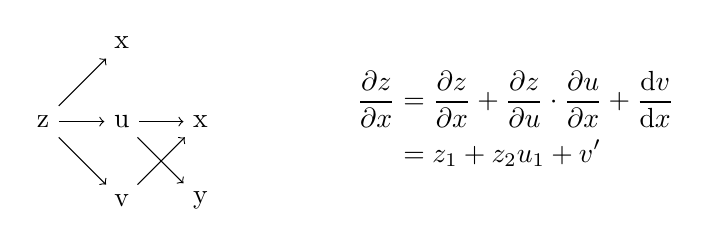
\begin{tikzpicture}
            \node (z) at (0, 0) {z};
            \node (X) at (1, 1) {x};
            \node (u) at (1, 0) {u};
            \node (v) at (1, -1) {v};
            \node (x) at (2, 0) {x};
            \node (y) at (2, -1) {y};
            \node (final) at (6, 0) 
            {$\begin{aligned}
                \frac{\partial z}{\partial x} &= \frac{\partial z}{\partial x} + 
                \frac{\partial z}{\partial u} \cdot \frac{\partial u}{\partial x} + 
                \frac{\dif v}{\dif x} \\
                &= z_1 + z_2 u_1 + v'
            \end{aligned}$};

            \draw[->] (z) -- (X);
            \draw[->] (z) -- (u);
            \draw[->] (z) -- (v);
            \draw[->] (u) -- (x);
            \draw[->] (u) -- (y);
            \draw[->] (v) -- (x);
        \end{tikzpicture}

        {\heiti 应用}：直线换元，作 $\varphi(t) = f(tx, ty, \cdots)$ 转为一元函数。

        隐函数求导：等式两侧同时求全微分，基于 Cramer 法则解方程。看作以各 $\dif x^i$ 为独立变量，满足附加方程。\\
        隐函数存在定理：（证明略，较复杂）
        $$\begin{cases}
            f_1(x^1, \cdots, x^m, \; y^1, \cdots y^n) &= 0 \\
            \vdots & \vdots \\
            f_m(x^1, \cdots, x^m, \; y^1, \cdots, y^n) &= 0
        \end{cases}$$
        在 $\mat{v}$ 处，$m$ 个 $n + m$ 元方程确定了 $n$ 个隐函数 $y^i = y^i(x^1, \cdots, x^m)$，若满足条件：\\
        a. $\forall f_i$ 均在 $\mat{v}_0$ 处有连续偏导；\\
        b. $\mat{v}$ 满足方程组；\\
        c. Jacobi 行列式 $\dfrac{\partial (f_1, \cdots, f_m)}{\partial (y^1, \cdots, y^n)} \neq 0$。
        （即系数行列式，在 Cramer 法则中做分母。）

        也可用向量值函数表示，证明略。这里值域维数应不少于隐函数个数。\\
        $\mat{x} = (x_1, \cdots, x_n)$，$\mat{y} = (y_1, \cdots, y_m)$，连续可微函数 $F(\mat{x}, \mat{y}): \Omega \subset \field{R}^{n + m} \to \field{R}^{m}$ 满足：\\
        a. $F(\mat{x}_0, \mat{y}_0) = \mat{0}$ \\
        b. $\det \Dif_{y} F(\mat{x_0}, \mat{y_0}) \neq 0$ \\
        则在 $(\mat{x_0}, \mat{y_0})$ 附近存在隐函数 $\mat{y} = y(\mat{x})$，且 $y(\mat{x})$ 在 $\field{R}^{n}$ 上也连续可微，并且
        $$\Dif y(\mat{x}) = -(\Dif_y F(\mat{x}, y(\mat{x})))^{-1} \, \Dif_x F(\mat{x}, y(\mat{x}))$$

        在 $x, y$ 均为一维的特例下，$\frac{\dif y}{\dif x} = -\frac{f_x}{f_y}$，与一般形式一致。

    \section{向量值函数微分}
    给矩阵赋范数，满足：\\
    a. $N(A) \geqslant 0 \; \land \; N(A) = 0 \iff A = \mat{0}$ \\
    b. $N(\lambda A) = |\lambda|N(A)$ \\
    c. $N(A + B) \leqslant N(A) + N(B)$ \\
    d. $N(AB) \leqslant N(A)N(B)$

    \begin{itemize}
        \item $\len{A} = \sqrt{\sum_i\sum_j a_{i, j}^2}$
        \item $|A| = \max_k\{ \sum_{i} |a_{k, i}| \}$ 绝对值和最大的一行
    \end{itemize}
    有 $\len{A\mat{x}} \leqslant \len{A}\len{\mat{x}}$，$|A\mat{x}| \leqslant |A||\mat{x}|$

        \subsection{导数与微分}
        定义由一元情景下的可微自然推广：$f(\mat{x + \Delta x}) - f(\mat{x}) = A\Delta\mat{x} + o(\len{\Delta\mat{x}})$。

        记定义域 $\Omega \subset \field{R}^m$，$f: \Omega \to \field{R}^n$。若{\heiti 矩阵} $A \in M^{n \times m}$ 满足：
        $$\lim_{\len{\Delta \mat{x}} \to 0} \frac{\len{f(\mat{x_0} + \Delta\mat{x}) - f(\mat{x_0}) - A\Delta\mat{x}}}{\len{\Delta \mat{x}}} = 0$$
        则定义导数 $\Dif f(\mat{x_0}) := A$。（此处，可导与可微等价。）

        本质依然为线性近似，一元的线性性进化为线性映射，而线性映射用矩阵描述。

        进一步地，可定义偏微分。任取一些维度的集合，不妨记 $\mat{x} = (\mat{x}, \mat{y})$，则 $\Dif_x F(\mat{x_0}, \mat{y}_0) := A$。这里把子空间整体视为变量。

        高阶微分需要张量，即（比矩阵）更高维的结构来描述，不讨论。

        \subsection{Jacobi 矩阵}
        Jacobi 矩阵：每一行，对每个自变量逐个求导；所有函数按列堆叠。
        $$J_f \, / \, \frac{\partial (f_1, \cdots, f_m)}{\partial (y_1, \cdots, y_n)} \; := \; \begin{pmatrix}
            \dfrac{\partial f_1}{\partial y^1} & \cdots & \dfrac{\partial f_m}{y^n} \\
            \vdots & \ddots & \vdots \\
            \dfrac{\partial f_m}{\partial y^1} & \cdots & \dfrac{\partial f_m}{\partial y^n}
        \end{pmatrix}$$

        Jacobi 行列式：Jacobi 矩阵的行列式，记为 $\dfrac{\partial (f_1, \cdots, f_m)}{\partial (y^1, \cdots, y^n)}$。（这既可表矩阵，亦可表行列式，依上下文确定。）

        Jacobi 矩阵即为 $f(\mat{x})$ 在一点的导数。\\
        证明：可微时，充要各分量 $f_i(\mat{x}): \field{R}^m \to \field{R}$ 均可微。而此时 $\dif f_i(\mat{x_0}) = \sum \frac{\partial f_i}{\partial x^i}(\mat{x_0})$，即 Jacobi 矩阵的一行。细节略。

        \subsection{法则}
        证明略。
        \begin{itemize}
            \item $\Dif (f \pm g) = \Dif f \pm \Dif g$
            \item $\Dif (u f) = u \Dif f + f\Dif u$，其中 $u: \field{R}^m \to \field{R}$ 为数量值函数。
            \item $\Dif \inner{f}{g} = (f)^T\Dif g + (g)^T\Dif f$，其中 $\inner{}{}$ 为向量内积/点乘。
            \item 对可叉乘向量，$\Dif (f \times g) = (\Dif f) \times g + f \times (\Dif g)$
            \item 链式法则：$\Dif (g \circ f) = \Dif f(g) \,\Dif f$
        \end{itemize}

        逆映射定理：若 $f: U \to V$ 是一个连续可微映射，$a \in U$ 满足 $\det \Dif f(a) \neq 0$，则在 $a$ 局部微分可微。即，$\exists U_0, V_0$，$f(U_0) = V_0$ 且 $f$ 在 $U_0$ 上是双射，并且逆映射 $f^{-1}$ 也是 $V_0$ 上的连续可微映射。\\
        证明：隐函数存在定理，略。

        逆映射求导：$\Dif f^{-1} = (\Dif f)^{-1}$，其中 $-1$ 表示逆矩阵。

        \subsection{中值不等式与偏微分}
        Lagrange 定理在高维退化为不等式：$\exists \mat{c} \in (\mat{a} \to \mat{b})$（这里指连接两点的直线段），$|f(\mat{b}) - f(\mat{a})| \leqslant |\Dif f(\mat{c})||\mat{b} - \mat{a}|$。其中这里任取一种范数（推广的切比雪夫/欧几里得）。\\
        证明：需要 Taylor 公式在一阶的情景（a.k.a. 有限增量公式），以及不等式技巧。

        偏微分：为左右两个子矩阵。证明基于定义简单推得。
        $$\Dif f(\mat{x_0}, \mat{y_0}) = \begin{pmatrix}
            \Dif_x f(\mat{x_0}, \mat{y_0}) \; \vdots \; \Dif_y f(\mat{x_0}, \mat{y_0})
        \end{pmatrix}_{(\mat{x_0}, \mat{y_0})}$$

    \section{Taylor 定理}
    这里只处理数量值函数的 Taylor 公式，向量值函数的高阶微分尚不能涉及，其 Taylor 公式亦略。

    使用{\heiti 多元转一元技巧}，记 $\varphi: [0, 1] \to \field{R}$，$\varphi(t) = f(\mat{x_0} + t\Delta\mat{x}) = f(x^1 + t\difx^1, \cdots, x^m + t\difx^m)$。对其使用 Maclaurin 公式， $\varphi(t) = \varphi(0) + \sum \frac{t^k}{k!} \varphi^{(k)}(0) + R$。
    
    $\varphi^{(k)}(t) = \frac{\dif}{\dif t} \varphi^{(k - 1)}(t) = \sum (\frac{\partial \varphi^{(k - 1)}(t)}{\partial x^i} \difx^i) \implies (\sum (\dif x^i) \frac{\partial}{\partial x^i})^k f(\mat{x_0} + t\Delta\mat{x})$。其中 $\difx^i$ 是第 $i$ 维度的变化（具体值），$\frac{\partial}{\partial x^i}$ 是求偏导。算子的结合按顺序表复合偏导，$\difx^i$ 作为常数乘之。

    $$T_n(\mat{x}) = \sum_{k = 0}^n \frac{1}{k!} \; (\sum_{i = 1}^{m} (\dif x^i) \frac{\partial}{\partial x^i})^k \; f(\mat{x_0}) + R(\mat{x})$$

    余项 $R(\mat{x})$，均展开到 $n$ 次项：
    \begin{itemize}
        \item Peano 余项 \\
            $R_n = o(\len{\mat{x - x_0}}^{n})$
        \item Lagrange 余项 \\
            $R_{n + 1} = \dfrac{1}{(n + 1)!}(\sum_{i = 1}^{m} (\dif x^i) \dfrac{\partial}{\partial x^i})^{n + 1} f(\mat{x_0} + \theta\Delta\mat{x})$
        \item 积分余项（仍然注意阶乘和幂次的不同） \\
            $R_{n + 1} = \dfrac{1}{n!}\int_{0}^{1} (1 - t)^n (\sum_{i = 1}^{m} (\dif x^i) \dfrac{\partial}{\partial x^i})^{n + 1} f(\mat{x_0} + t \Delta\mat{x}) \,\dif t$
    \end{itemize}

    \section{函数性质研究}
    显然极值/最值仅能对数量值函数讨论。

        \subsection{无约束极值}
        定义由一维自然推广，易知只能对内点下定义。

        必要，使用一阶导：$\forall i, \; \frac{\partial}{\partial x^i} f = 0 \; \iff \; \nabla f = \mat{0}$ \\
        $\nabla f = \mat{0}$ 的点亦称驻点。\\
        证明：用 Peano 余项展开，若非零，则一阶偏导系数占主导，$\mat{x_0} \pm \Delta\mat{x}$ 必非零且异号。

        为利用二阶导判断，Taylor 展开，其中一阶部分全零：$\Delta f = (\sum_{i} \difx^i \frac{\partial}{\partial x^i})^2 f(\mat{x_0}) + o(\rho^2)$

        符号由二阶导主导，由此定义 Hesse 矩阵 $H_f$：
        $$H_f := \begin{pmatrix}
            \frac{\partial^2}{\partial x^1 \partial x^1} f & \cdots & \frac{\partial^2}{\partial x^1 \partial x^m} f \\
            \vdots & \ddots & \vdots \\
            \frac{\partial^2}{\partial x^m \partial x^1} f & \cdots & \frac{\partial^2}{\partial x^m \partial x^m} f
        \end{pmatrix}$$
        则 $f(\mat{x_0} + \Delta\mat{x}) - f(\mat{x_0}) = (\Delta\mat{x})^T H_f(\mat{x_0}) (\Delta\mat{x})$，为关于 $\Delta\mat{x}$ 的二次型。

        充分，使用二阶导：
        \begin{itemize}
            \item $H_f(\mat{x_0})$ 正定：$\mat{x_0}$ 为严格极小值 \\
                所有顺序主子式为正：$\forall i$, $\det \begin{pmatrix}
                    f_{11} & \cdots & f_{1i} \\
                    \vdots & \ddots & \vdots \\
                    f_{i1} & \cdots & f_{ii}
                \end{pmatrix} > 0$
            \item $H_f(\mat{x_0})$ 负定：$\mat{x_0}$ 为严格极大值 \\
                $-f$ 为极小值，即 $H_f$ 矩阵所有系数取反后行列式恒正：$\forall i$, $(-1)^i \det \begin{pmatrix}
                    f_{11} & \cdots & f_{1i} \\
                    \vdots & \ddots & \vdots \\
                    f_{i1} & \cdots & f_{ii}
                \end{pmatrix} > 0$，即偶正奇负。
            \item $H_f(\mat{x_0})$ 不定：必不为极值
        \end{itemize}
        正定矩阵判定见线性代数，若把正/负定改为半正/负定，则为对应的非严格极值。

        \subsection{有约束极值}
        Lagrange 乘数法

        在限制 $\varphi_{1 \sim m}$ 下，求 $f$ 的极值。这里限制满足正则条件：$\varphi_{1 \sim m}$ 的 Jacobi 矩阵的秩恰为 $m$，意即这 $m$ 个限制彼此独立，排除平凡情况。
        $$\begin{matrix}
            \max/\min f(x_1, \cdots, x_n, y_1, \cdots, y_m) & \\
            \text{s.t.} \begin{cases}
                \varphi_1(x_1, \cdots, x_n, y_1, \cdots, y_m) &= 0 \\
                \vdots & \vdots \\
                \varphi_m(x_1, \cdots, x_n, y_1, \cdots, y_m) &= 0
            \end{cases} &
            \quad\text{ensure }\mathrm{rank} \dfrac{\partial (\varphi_1, \cdots, \varphi_m)}{\partial (y_1, \cdots, y_m)} = m
        \end{matrix}$$

        不妨认为，存在隐函数 $\forall j = 1 \sim m$，$y_i = \psi(x_1, \cdots, x_n)$。（其存在性依赖正则条件。对变量进行适量的重编号，总可以选出 $\{y_m\}$ 使对它们的 Jacobi 矩阵满秩/行列式不为零，进而使用隐函数存在定理。）

        另记 $g(x_1, \cdots, x_n) = f(x_1, \cdots, x_n, \psi_1(\{x_n\}), \cdots, \psi_m(\{x_n\}))$，问题完全归为 $g$ 的极值点，于是必要限制 $\nabla g = \mat{0}$。对每个 $x_i$ 求偏导得：
        $$\forall i = 1 \sim n \quad \frac{\partial f}{\partial x_i} + \sum_{j = 1}^{m} \frac{\partial f}{\partial y_j} \, \frac{\partial \psi_j}{\partial x_i} = 0$$

        再对约束条件求偏导：
        $$\forall i = 1 \sim n \; \forall t = 1 \sim m \quad \frac{\partial \varphi_t}{\partial x_i} + \sum_{j = 1}^{m} \frac{\partial \varphi_t}{\partial y_j} \, \frac{\partial \psi_j}{\partial x_i} = 0$$

        显然隐函数总是难以显化的，考虑避免之。选定一组特定的 $\{\lambda_m\}$，分别乘以 $m$ 个约束条件，使得加上 $\nabla f$ 后消去 $\frac{\partial \psi}{\partial x}$。这里对 $n$ 个自由元 $\{x_n\}$ 均做消元，代入后共 $m \times m$ 个 $\frac{\partial \varphi_t}{\partial y_j} \, \frac{\partial \psi_j}{\partial x_i}$，外层按 $y_j$ 整理，从每个约束的偏导中抽出一个。
        $$\forall i = 1 \sim n \quad \boxed{\frac{\partial f}{\partial x_i} + \sum_{t = 1}^{m} \lambda_t \frac{\partial \varphi_t}{\partial x_i}}  + \sum_{j = 1}^{m} (\boxed{\frac{\partial f}{\partial y_j} + \sum_{t = 1}^{m} \lambda_t\frac{\partial \varphi_t}{\partial y_j}}  )\frac{\partial \psi_j}{x_i} = 0$$
        发现 $\{\lambda_m\}$ 需满足的式子与 $\{x_n\}$ 无关，因此有解即对所有式子均适用。此外，最初对 $\{y_m\}$ 的合理选取使得 Jacobi 行列式 $\frac{\partial(\varphi_1, \cdots, \varphi_m)}{\partial (y_1, \cdots, y_m)} \neq 0$，于是该线性方程组必有唯一解 $\{\lambda_m\}$。

        称 $\{\lambda_m\}$ 为 Lagrange 乘数，定义 Lagrange 函数 $F$，统一了所有条件：$\nabla F = \mat{0}$
        $$\begin{matrix}
            F(x_1, \cdots, x_n, y_1, \cdots, y_m, \lambda_1, \cdots, \lambda_m) := f + \sum\limits_{t = 1}^{m} \lambda_t \varphi_t \\
            \text{s.t.} \begin{cases}
                \dfrac{\partial F}{\partial x_i} &= \dfrac{\partial f}{\partial x_i} + \sum\limits_{t = 1}^{m} \lambda_t \dfrac{\partial \varphi_t}{\partial x_i} = 0 \quad \forall i = 1 \sim n \\
                \dfrac{\partial F}{\partial y_j} &= \dfrac{\partial f}{\partial y_j} + \sum\limits_{t = 1}^{m} \lambda_t \dfrac{\partial \varphi_t}{\partial y_j} = 0 \quad \forall j = 1 \sim m\\
                \dfrac{\partial F}{\partial \lambda_t} &= \varphi_t = 0
            \end{cases}
        \end{matrix}$$

        在 Lagrange 函数的{\heiti 驻点}中排查极值点。Lagrange 函数的极值点必为 $g$ 的极值点，反之 $g$ 的极值点可能仅为 Lagrange 函数的驻点。

        必然不会遗漏解。因为 $\{\lambda_m\}$ 由各变量与偏导唯一确定，并且一定满足 $\nabla F = \mat{0}$。

        几何理解：$\nabla F = \nabla f + \sum \lambda_t \nabla \varphi_t = 0$，即在极值点处，$f$ 的切向量在各限制条件的切向量张成的子空间内。特别地，二维下且 $m = 1$ 时，曲线 $f = \text{Ans}$ 与 $\varphi = 0$ 必相切，则二者的法向量共线 $\nabla f = \mu \nabla \varphi$，导出了 $\lambda$。高维下的几何理解尚不明确。

        \subsection{最值}
        从驻点、偏导不存在的点、边界中取最值。

        有约束也仅是改为 Lagrange 函数的驻点。

    \section{低维微分几何}
        \subsection{曲线}
        表示形式：\\
        a. 参数方程：$\mat{r} = \mat{r}(t)$ \\
        b. 曲面的交/隐函数：$\begin{cases}
            F(x, y, z) &= 0 \\
            G(x, y, z) &= 0
        \end{cases}$

        规定曲线的正向为参数 $t$ 增大的方向，切向量方向也规定与曲线方向一致。

        切线是自然的研究对象，法平面是其副产物。正如物理引入自然坐标系一样，以曲线为基础构建坐标系或将带来方便，这即 Frenet 标架。为此，需先讨论自然参数。它由弧长引入，借此得以摆脱参数 $t$，完全用曲线描述曲线。

        \subsubsection{切线}
        \begin{itemize}
            \item[-] 参数方程 \\
            切线为割线的极限，只关心方向，除 $\Delta t$ 无影响：$\mat{v} = \lim \frac{\mat{r}(t) - \mat{r}(t_0)}{t - t_0}$。于是：\\
            切向量：
            $$\mat{n} = \frac{\dif \mat{r}}{\dif t} = (x'(t_0), y'(t_0), z'(t_0))$$
            切线方程：
            $$\frac{x - x_0}{x'(t_0)} = \frac{y - y_0}{y'(t_0)} = \frac{z - z_0}{z'(t_0)}$$
            
            \item[-] 隐式表示 \\
            基于隐函数求导可得 $\dif x, \dif y, \dif z$ 的比例关系，可得 $\mat{n}$。此外，总有参数形式解存在，对 $t$ 求导得 $F_x x'(t) + F_y y'(t) + F_z z'(t) = G_x x'(t) + G_y y'(t) + G_z z'(t) = 0$，因此 $\nabla F, \nabla G \bot \mat{n}$。于是切向量：
            $$\mat{n} = \nabla F_{\mat{r}_0} \times \nabla G_{\mat{r}_0} = \begin{vmatrix}
                \mat{i} & \mat{j} & \mat{k} \\
                F_x(\mat{r}_0) & F_y(\mat{r}_0) & F_z(\mat{r}_0) \\
                G_x(\mat{r}_0) & G_y(\mat{r}_0) & G_z(\mat{r}_0)
            \end{vmatrix}$$

            对第一行展开得切线方程：
            $$\dfrac{x - x_0}{\frac{\partial (F, G)}{\partial (y, z)}|_{\mat{r_0}}} = \dfrac{y - y_0}{\frac{\partial (F, G)}{\partial (z, x)}|_{\mat{r_0}}} = \dfrac{z - z_0}{\frac{\partial (F, G)}{\partial (x, y)}|_{\mat{r_0}}}$$
        \end{itemize}

        \subsubsection{法平面}
        法平面为该点处垂直与切线的平面，故法平面方程：
        $$(\mat{r} - \mat{r_0}) \cdot \mat{n} = 0$$

        \subsubsection{弧长}
        $$\dif s = \len{\mat{r}'(t)} \,\dif t = \sqrt{[x'(t)]^2 + [y'(t)]^2 + [z'(t)]^2} \,\dif t = \sqrt{(\dif x)^2 + (\dif y)^2 + (\dif z)^2}$$

        弧长定义为各小线段和的极限，弧微分 $\dif s$。依 Lagrange 中值定理知 $\dif x = x'(\xi)\,\dif t$，同理 $y, z$ 分别有 $\eta, \zeta$。使用同一个变元 $\xi$ 以构成积分，不等式限制误差。或当 $\Delta\mat{r} \to 0$ 时 $\xi, \eta, \zeta$ 彼此接近，严谨性未知。

        {\heiti 特别地}，对平面曲线 $\dif z \equiv 0$：\\
        a. $y = y(x)$：$\dif s = \sqrt{1 + [y'(x)]^2} \difx$ \\
        b. 极坐标 $\rho = \rho(\theta)$：$\dif s = \sqrt{[\rho(\theta)]^2 + [\rho'(\theta)]^2} \,\dif\theta$

        \subsubsection{自然参数}
        $s$ 必然单调递增，故存在双射 $s \leftrightarrow t$，进而存在 $\mat{r} = \mat{r}[t(s)]$。称 $s$ 为曲线的自然参数。换言之，存在 $\mat{r} = \mat{r}(s)$，这意味着可以通过曲线自身描述曲线。

        考虑到 $(\dif s)^2 = (\dif x)^2 + (\dif y)^2 + (\dif z^2) \implies 1 = (\frac{\dif x}{\dif s})^2 + (\frac{\dif y}{\dif s})^2 + (\frac{\dif z}{\dif s})^2$，故以此为参数的切向量为{\heiti 单位向量}：
        $$\mat{n} = \frac{\dif \mat{r}}{\dif s} = (\frac{\dif x}{\dif s}, \frac{\dif y}{\dif s}, \frac{\dif z}{\dif s})$$

        \subsubsection{Frenet 标架}
        记 $\mat{r}'(s) := \frac{\dif \mat{r}}{\dif s}$，$\mat{r}'(t) := \frac{\dif \mat{r}}{\dif t}$

        {\heiti 引理}：对向量 $\mat{u}(t), \, \mat{v}(t)$，其内积与外积求导与乘积求导形式相同（{\heiti 叉乘应保持顺序}）。证明只需按坐标形式展开并整理。（这也可见于向量值函数的求导。）\\
        a. $(\mat{u} \cdot \mat{v})' = \mat{u}' \cdot \mat{v} + \mat{u} \cdot \mat{v}'$ \\
        b. $(\mat{u} \times \mat{v})' = \mat{u}' \times \mat{v} + \mat{u} \times \mat{v}'$

        {\heiti 引理}：对恒为单位向量的 $\mat{e}(t)$，其导数 $\mat{e}'(t_0) \bot \mat{e}(t_0)$，大小为角速度。画图知显然。\\
        进一步地，这导数反映了 $\mat{e}$ 的转动程度，由此将引出曲率 $\kappa$ 与挠率 $\tau$。

        对一组正交基，可以{\heiti 使用点乘提取坐标}。

        \begin{itemize}
            \item 切向量 $\mat{T}(s)$ \\
                $\mat{r}'(s) = \mat{r}'(t) \cdot \frac{\dif t}{\dif s} = \mat{r}'(t) (\frac{\dif s}{\dif t})^{-1} = \frac{\mat{r}'(t)}{\len{\mat{r}'(t)}}$ 为单位向量。记
                $$\mat{T}(s) := \mat{r}'(s)$$
            \item 主法线向量 $\mat{N}(s)$ \\
                对 $\mat{T}(s)$ 进一步求导，因其为单位向量，故 $\mat{T}'(s) \bot \mat{T}$。这即是 $\mat{N}(s)$ 的方向。\\
                此外，$\len{\mat{T}'(s)} = |\frac{\dif \theta}{\dif s}|$ 为角度的变化率。定义曲率 $k(s) := \len{\mat{T}'(s)} = \lim |\frac{\dif \theta}{\dif s}|$ \\
                在曲率 $\kappa(s) \neq 0$ 的地方，记
                $$\mat{N}(s) := \frac{\mat{T}'(s)}{\len{\mat{T}'(s)}} = \frac{\mat{r}''(s)}{\len{\mat{r}''(s)}}$$
            \item 次法线向量 $\mat{B}(s)$ \\
                已确定两个方向，叉乘即得第三轴。
                $$\mat{B}(s) := \mat{T}(s) \times \mat{N}(s)$$
        \end{itemize}

        \begin{tikzpicture}
            \pgfmathsetmacro{\length}{4}
            \pgfmathsetmacro{\ang}{30}
            \pgfmathsetmacro{\verconst}{0.5} % AE / AD
            \pgfmathsetmacro{\horconst}{0.25} % AI / AB

            \coordinate (A) at (0, 0);
            \coordinate (B) at ($(A) + (\length, 0)$);
            \coordinate (C) at ($(B) + (\ang:\length)$);
            \coordinate (D) at ($(A) + (\ang:\length)$);

            \coordinate (E) at ($(A)!\verconst!(D)$);
            \coordinate (F) at ($(B)!\verconst!(C)$);
            \coordinate (G) at ($(F) + (0, \length)$);
            \coordinate (H) at ($(E) + (0, \length)$);

            \coordinate (I) at ($(A)!\horconst!(B)$);
            \coordinate (J) at ($(D)!\horconst!(C)$);
            \coordinate (K) at ($(J) + (0, \length)$);
            \coordinate (L) at ($(I) + (0, \length)$);

            \path [name path = EF] (E) -- (F);
            \path [name path = IJ] (I) -- (J);
            \path [name intersections = {of = EF and IJ, by = P}];

            \path [name path = GH] (G) -- (H);
            \path [name path = KL] (K) -- (L);
            \path [name intersections = {of = GH and KL, by = Q}];

            \path [name path = DA] (D) -- (A);
            \path [name path = LI] (L) -- (I);
            \path [name intersections = {of = DA and LI, by = X}];

            \path [name path = HE] (H) -- (E);
            \path [name intersections = {of = KL and HE, by = Y}];

            \path [name path = JK] (J) -- (K);
            \path [name intersections = {of = GH and JK, by = Z}];

            \path [name path = CD] (C) -- (D);
            \path [name path = FG] (F) -- (G);
            \path [name intersections = {of = CD and FG, by = W}];

            \draw (P) node [above left] {P};
            \draw (I) node [below] {$\mat{T}(s)$};
            \draw (F) node [below right] {$\mat{N}(s)$};
            \draw (Q) node[above left] {$\mat{B}(s)$};

            \draw [->, black] (P) -- node[below, rotate = \ang, pos = 0.3]{切线} (I);
            \draw [dashed, black] (P) -- (J);
            \draw [->, black] (P) -- node[below]{主法线} (F);
            \draw [dashed, black] (P) -- (E);
            \draw [->, black] (P) -- node[below, pos = 0.6, rotate = 90]{次法线} (Q);

            \draw [red] (A) -- node[below, pos = 0.8]{密切平面} (B) -- (C) -- (W);
            \draw [dashed, red] (W) -- (D) -- (X);
            \draw [red] (X) -- (A);

            \draw [green!40!black!60] (F) -- node[above, pos = 0.8, rotate = 90]{法平面} (G) -- (H) -- (Y);
            \draw [dashed, green!40!black!60] (Y) -- (E);

            \draw [dashed, blue] (J) -- (Z);
            \draw [blue] (Z) -- (K) -- (L) -- node[right, pos = 0.2]{\rotatebox{90}{从切平面}} (I);

            \coordinate (s) at ($(P) + 0.8*(40:\length)$);
            \coordinate (t) at ($(P) + 0.3*(-40:\length)$);
            \draw [black, thick] (s) .. controls ($(P) - 0.1*(\length, 0)$) .. (t);
        \end{tikzpicture}

        $(\mat{T}, \mat{N}, \mat{B})$ 两两垂直且为单位向量，其方向随着曲线的运动而改变。称 Frenet 标架 / 活动标架。$\mat{T}, \mat{N}, \mat{B}$ 依次对应于 x, y, z，为右手系。

        对一组规范正交标架 $\{\mat{e}_3(t)\}$，用其描述导数 $\mat{e}'_i(t) = \sum \omega_{i, j} \mat{e}_j$。利用 $\mat{e}_i \cdot \mat{e}_j = [i = j]$ 左右对 $t$ 求导，可以证明 $\{\omega_{3, 3}\}$ 反对称，即 $\omega_{i, j} = -\omega_{j, i}$。将结论应用于 Frenet 标架，并已知 $\mat{T}'(s) = \kappa\mat{N}(s)$，于是：（这里 $\tau$ 为一系数）
        $$\text{Frenet 公式} \quad \begin{cases}
            \begin{matrix}
                \mat{T}'(s) & = &                    & \kappa \mat{N} & \\
                \mat{N}'(s) & = & -\kappa \mat{T} &                   & +\tau \mat{B} \\
                \mat{B}'(s) & = &                    & -\tau \mat{N}  &
            \end{matrix}
        \end{cases}$$
        发现 $\mat{B}'(s) \,//\, \mat{N}(s)$。另一解读：$\mat{B}'(s) = \mat{T}'(s) \times \mat{N}(s) + \mat{T}(s) \times \mat{N}'(s)$。而 $\mat{T}'(s)$ 与 $\mat{N}(s)$ 共线，故化简为 $\mat{B}'(s) = \mat{T}(s) \times \mat{N}'(s)$。于是 $\mat{B}'(s) \bot \mat{T}$，另由前知 $\mat{B}'(s) \bot \mat{B}$，则其必然平行于 $\mat{N}$。

        定义挠率 $\tau := -\mat{B}(s) \cdot \mat{N}(s)$，由前式左右同时点乘 $\mat{N}$ 解得。

        解读：
        \begin{itemize}
            \item 密切平面 \\
                有泰勒公式 $\mat{r}(t_0) = \sum_{k = 0}^{n} \frac{(t - t_0)^k}{k!} \mat{r}^{(k)}(t_0) + \mat{R}_{n + 1}(t)$，其中余项 $\mat{R}_{n + 1}(t)$ 满足 $t \to t_0$ 时趋近于 $\mat{0}$。亦可记为 $o(|t - t_0|^n)$。证明：按分量展开。\\
                而 $\mat{r}'(s_0) = \mat{T}, \, \mat{r}''(s_0) = \kappa\mat{N}$，于是
                $$\mat{r}(s) = \mat{r}(s_0) + (s - s_0)\boxed{\mat{T}(s_0)} + \frac{(s - s_0)^2}{2}\kappa\boxed{\mat{N}(s_0)} + o((s - s_0)^2)$$
                密切平面由 $\mat{T}, \mat{N}$ 张成，而以该平面近似曲面时，误差为二阶无穷小。这是能取得的最好结果，故以“密”称。
            \item 曲率 \\
                描述切线的扭动程度。
                $$\kappa(s) := \len{\mat{T}'(s)}$$
            \item 挠率 \\
                描述密切平面的扭动程度，即曲线在多大程度上偏离平面曲线。副法线向量 $\mat{B}$ 为密切平面的法向量，故以其为代表。
                $$|\tau(s)| = \len{\mat{B}'(s)}$$
        \end{itemize}

        按 $\mat{r}$ 整理，所有向量均为以 $s$ 为参数的函数：
        \begin{longtable}[h]{l l l l r r r}
            $\mat{r}'(s)$ & = & & = & $\mat{T}$ & & \\
            $\mat{r}''(s)$ & = & $(\mat{T})'$ & = & & $\kappa \mat{N}$ & \\
            $\mat{r}'''(s)$ & = & $(\kappa \mat{N})' = \kappa' \mat{N} + \kappa \mat{N}'$ & = & $-\kappa^2 \mat{T}$ & $+ \frac{\dif\kappa}{\dif s} \mat{N}$ & $+\kappa \tau \mat{B}$
        \end{longtable}

        于是有（其中 $\mat{r}'(s) \times \mat{r}''(s) = \kappa \mat{T} \times \mat{N} = \kappa \mat{B}$）
        $$\begin{cases}
            \kappa &= \boxed{\len{\mat{r}''(s)}} \\
            \tau &= \dfrac{\mat{r}'''(s) \cdot \mat{B}}{\kappa} = \dfrac{\mat{r}'''(s) \cdot (\mat{r}'(s) \times \mat{r}''(s))}{\kappa^2} = \boxed{\dfrac{[\mat{r}'(s) \, \times \, \mat{r}''(s)] \, \cdot \, \mat{r}'''(s)}{\len{\mat{r}''(s)}^2}}
        \end{cases}$$

        对于以参数 $\mat{r} = \mat{r}(t)$ 表示的曲线，利用链式法则展开，并使用 $\kappa = \len{\mat{r}'(s) \times \mat{r}''(s)}$ 得
        $$\begin{cases}
            \kappa(t) &= \dfrac{\len{\mat{r}'(t) \times \mat{r}''(t)}}{\len{\mat{r}'(t)}^3} \\
            \tau(t) &= \dfrac{[\mat{r}'(t) \times \mat{r}''(t)] \cdot \mat{r}'''(t)}{[\mat{r}'(t) \times \mat{r}''(t)]^2}
        \end{cases}$$

        \subsubsection{曲率}
        $$\kappa(t) = \boxed{\len{\mat{r}''(s)}} = \frac{\len{\mat{r}'(t) \times \mat{r}''(t)}}{\len{\mat{r}'(t)}^3}$$

        称 $\kappa = 0$ 的点为平直点。

        曲率半径 $\rho := \frac{1}{\kappa}$。规定 $\kappa = 0$ 时 $\rho = +\inf$：直线。
        
        曲率圆圆心 $\mat{r}_O = \mat{r}(s_0) + \rho \mat{N}(s_0)$：主法线向量 $\mat{N}$ 总指向曲线凹侧。

        特别地，对平面曲线 $x = x(t), y = y(t)$ 或 $y = y(x)$ 有：
        $$\kappa = \frac{|x'(t)y''(t) - x''(t)y'(t)|}{[(x'(t))^2 + (y'(t))^2]^{\frac{3}{2}}} = \frac{|y''(x)|}{[1 + (y'(x))^2]^{\frac{3}{2}}}$$

        \subsubsection{挠率}
        $$\tau(t) = \dfrac{[\mat{r}'(s) \, \times \, \mat{r}''(s)] \, \cdot \, \mat{r}'''(s)}{\len{\mat{r}''(s)}^2} = \dfrac{[\mat{r}'(t) \times \mat{r}''(t)] \cdot \mat{r}'''(t)}{[\mat{r}'(t) \times \mat{r}''(t)]^2}$$

        对于没有平直点的曲线，其为平面曲线的充要条件是 $\tau \equiv 0$。\\
        证明：必要显然。充分，$\tau \equiv 0$ 则 $\mat{B} \equiv \mat{B_0}$ 为常向量。构造 $\varphi(s) = \mat{r}(s) \cdot \mat{B}_0$，则 $\varphi'(s) = \mat{T} \cdot \mat{B}_0 \equiv 0$，故 $\mat{r}(s) \cdot \mat{B}_0 = \text{Const} \implies (\mat{r}(s) - \mat{r}(s_0)) \cdot \mat{B}_0 = 0$，即以 $\mat{B}_0$ 为法向量的一张平面。

        \subsection{曲面}
        表示形式：\\
        a. 参数方程：$\mat{r} = \mat{r}(u, v)$。
        限制 $u, v$ 为独立变量，也即 $\text{rank } \frac{\partial (x, y, z)}{\partial (u, v)} = 2$。这进一步说明，$\mat{r}_u \times \mat{r}_v \neq 0$（否则矩阵两列线性相关）。\\
        b. 隐函数：$F(x, y, z) = 0$

        曲面的研究内容远少于曲线，这里按形式分类，讨论法向量与切平面。

        \subsubsection{参数方程}
        考虑任一曲线 $u = u(t), v = v(t)$，由自然参数知这形式必然存在。对其求切线：$\frac{\dif \mat{r}}{\dif t} = \frac{\dif \mat{r}(u, v)}{\dif t} = \mat{r}_u \frac{\dif u}{\dif t} + \mat{r}_v\frac{\dif v}{\dif t}$，于是知其在 $\mat{r}_u$ 和 $\mat{r}_v$ 张成的平面上。

        切平面：过一点 $\mat{r}_0$ 的所有曲线的切线所经过的平面。\\
        法线：切平面在该点的法线。

        法向量可取为
        $$\mat{n} = \mat{r}_u \times \mat{r}_v$$
        
        则切平面方程：
        $$(\mat{r} - \mat{r}_0) \cdot (\mat{r}_u \times \mat{r}_v) = 0$$
        
        这是向量的混和积，于是有行列式表示 $\begin{vmatrix}
            (x - x_0) & (y - y_0) & (z - z_0) \\ 
            x_u (u_0, v_0) & y_u (u_0, v_0) & z_u (u_0, v_0) \\
            x_v (u_0, v_0) & y_v (u_0, v_0) & z_v (u_0, v_0)
        \end{vmatrix} = 0$。
        对第一行展开，得 \\
        法线方程：
        $$\dfrac{x - x_0}{\frac{\partial (y, z)}{\partial (u, v)}|_{\mat{r_0}}} = \dfrac{y - y_0}{\frac{\partial (z, x)}{\partial (u, v)}|_{\mat{r_0}}} = \dfrac{z - z_0}{\frac{\partial (x, y)}{\partial (u, v)}|_{\mat{r_0}}}$$

        {\heiti 特别地}：显式表示 $z = z(x, y)$，视为 $u = x, v = y, \mat{r} = (x, y, z(x, y))$ \\
        法向量：$\mat{n} = (1, 0, z_x) \times (0, 1, z_y) = (-z_x, -z_y, 1)$ \\
        法线：$\frac{x - x_0}{z_x} = \frac{y - y_0}{z_y} = \frac{z - z_0}{-1}$ \\
        切平面：$z - z_0 = z_x(x - x_0) + z_y(y - y_0)$（这可视为以切平面近似曲面，以直代曲。）

        \subsubsection{隐函数}
        对隐函数 $F(x, y, z) = 0$ 给出的曲面，如法炮制：记有曲线 $\mat{r} = \mat{r}(t)$，则 $F(x(t), y(t), z(t)) = 0$。对其求导得 $F_x x'(t) + F_y y'(t) + F_z z'(t) = 0$，即 $(F_x, F_y, F_z) \bot (x'(t), y'(t), z'(t))$。而垂直于任意切线的向量即该点的法向量。于是：

        法向量：
        $$\mat{n} = \nabla F (x_0, y_0, z_0)$$

        切平面：
        $$(\nabla F) \cdot (\mat{r} - \mat{r}_0) = 0$$

        从几何上，梯度为数值变化最大的方向，因此必然垂直于等值线。
    
    \chapter{多元函数积分}
    \section{重积分}
        本质上，重积分只能转化为累次积分求解。对区域割补，之后找到一个逐维扫描的方式，以此构建累次积分。

        先 $x$ 后 $y$：内层 $x$，外层 $y$，$\int \dif y \int_{y_l}^{y_r} \dif x$

        特别地，积不出的积分应放在外层，以冀内层结果能凑出可积的形式。

        \subsection{定义}
        $\field{R}^n$ 上的闭方块 $Q = \prod [a_i, b_i]$，记其体积 $\text{Vol}(Q) := \prod (b_i - a_i)$。记分割 $P$ 的模 $|P| := \max_{Q} \max \Delta_i$，即所有方块的最大棱长。定义
        $$\underbrace{\int \cdots \int}_{n} f(x^1, \cdots, x^n) \sdif (x^1, \cdots, x^n) = \int_{(\Omega)} f(\mat{x}) \sdif \Omega := \lim_{|P| \to 0} \sum f(\mat{x_i}) \text{Vol}(Q_i)$$

        其中，记 $(\Omega)$ 为积分区域，$\Omega$ 为此形体的度量。

        \subsection{可积}
        $f \in C\left( (\Omega) \right)$，即连续函数可积。

        \subsection{性质}
        下述 $(\Omega)$ 均为闭方块。开方块属于广义积分的问题。

        \begin{itemize}
            \item 线性：$\int_{(\Omega)} (\alpha f + \beta g) \sdif \Omega = \alpha \int_{(\Omega)} f \sdif \Omega + \beta \int_{(\Omega)} g \sdif \Omega$
            \item 区域可拆：$(\Omega) = (A) \cup (B) \,\land\, (A) \cap (B) = \emptyset$，则 $\int_{(\Omega)} = \int_{(A)} + \int_{(B)}$
            \item 保序：$f \leqslant g$，$\int_{(\Omega)} f \sdif\Omega \leqslant \int_{(\Omega)} g \sdif\Omega$ \\
                推论：$m \Omega \leqslant \int_{(\Omega)} f\sdif\Omega \leqslant M\Omega$，$|\int_{(\Omega)} f\sdif\Omega| \leqslant \int_{(\Omega)} |f|\sdif\Omega$ \\
                {\heiti 应用}：估值
            \item 积分中值定理：$f$ 在 $(\Omega)$ 上连续，则 $\exists \xi \in (\Omega)$，$\int_{(\Omega)} f\sdif\Omega = f(\xi)\Omega$
            \item {\heiti 对称性}：注意积分区域的对称性/字母的轮换对称性；被积函数的奇偶性 etc. 抵消。
        \end{itemize}

        \subsection{换元法}
        若连续可微映射 $\varphi: (E) \to \field{R}^n$，满足：\\
        a. $\forall t \in \text{int}(E)$，$\det \Dif \varphi(t) \neq 0$ \\
        b. $\varphi$ 在 $\text{int}(E)$ 上是单射。\\
        则
        $$\int_{\varphi((E))} f(\mat{x})\sdif\mat{x} = \int_{(E)} f(\varphi(t)) \,|\det \Dif \varphi(t)|\, \sdif t$$

        也即 $|\det \Dif \varphi(t)| = \frac{\partial(x^1, \cdots, x^n)}{\partial (t^1. \cdots, t^m)}$。

        常用计算：
        \begin{longtable}[h]{c | c | w{c}{10cm}}
            极坐标 & $\begin{cases}
                x = \rho \cos\theta \\
                y = \rho \sin\theta
            \end{cases}$ & $\begin{aligned}
                \dif l &= \rho \sdif\theta \quad (\rho \equiv r) \\
                \dif s &= \rho \sdif\rho \sdif\theta
            \end{aligned}$ \\
            \midrule
            球 & $z = \sqrt{r^2 - x^2 - y^2}$ & $\begin{aligned}
                \dif s &= \frac{r}{\sqrt{r^2 - x^2 - y^2}} \sdif x \sdif y \\
                 &= 2 \pi r \sdif z \\
                \dif V &= \pi (r^2 - z^2) \sdif z 
            \end{aligned}$ \\
            \midrule
            球面坐标 & $\begin{cases}
                x = \rho \sin\varphi \cos\theta \\
                y = \rho \sin\varphi \sin\theta \\
                z = \rho \cos\theta
            \end{cases}$ & $\begin{aligned}
                \dif s &= \rho^2 \sin\varphi \sdif\theta \sdif\varphi \\
                \dif V &= \rho^2 \sin\varphi \sdif\rho \sdif\theta \sdif\varphi
            \end{aligned}$ \\
            \midrule
            柱面坐标 & $\begin{cases}
                x = \rho \cos\theta \\
                y = \rho \sin\theta \\
                z = z
            \end{cases}$ & $\begin{aligned}
                \dif s &= \rho \sdif\theta \sdif z \quad (\rho \equiv r) \\
                \dif V &= \rho \sdif\rho \sdif\theta \sdif z
            \end{aligned}$
        \end{longtable}

        证明：求 Jacobi 行列式，或用几何近似：\\
        a. 极坐标近似为上底 $\rho\sdif\theta$，下底 $(\rho + \dif\rho)\sdif\theta$，腰 $\dif\rho$ 的等腰梯形（扇环）。\\
        b. 球面坐标近似为长 $\rho\sdif\varphi\sdif\theta$，宽 $\rho\sdif\varphi$，纵深 $\dif\rho$ 的长方体。\\
        也可更精细地近似（如棱台替换长方体），只需保留到 2 阶 / 3 阶无穷小，与维度一致。

        球面任意高度处环带面积为常数 $2 \pi r \sdif z$。\\
        证明：切开近似为矩形，长 $2 \pi \sqrt{r^2 - z^2}$。其在 z 轴的投影长度为 $\dif z$，但其与实际的高的差不可忽略。考虑任一点处的法向量 $\mat{n} = (x, y, z)$，其与 z 轴夹角 $\theta$ 满足 $\cos\theta = z/r$，而实际的高投影到 $\dif z$ 上，系数为 $\sin\theta = \frac{\sqrt{r^2 - z^2}}{r}$，于是 $\dif s = 2 \pi \sqrt{r^2 - z^2} (\sin\theta)^{-1}\sdif z = 2 \pi r \sdif z$

        $\varphi$ 为 $\rho$ 与 $z$ 轴夹角。\\
        椭球类考虑广义的极坐标变换，$\dif s = ab \rho \sdif\rho \sdif\theta$。\\
        形如 $(x - a)^2 + y^2 = a^2$，采用极坐标换元，$\theta \in [-\frac{\pi}{2}, \frac{\pi}{2}]$，$\rho \in [0, 2a\cos\theta]$

        为获得变量范围，考虑联立曲面方程。

        \subsection{含参变量的重积分}
        此处讨论含参变量积分的性质，为累次积分可换序做了分析的证明，最后给出普适的积分函数求导。

        限定在二维平面上，取定义域 $D = [a, b] \times [c, d]$，满足 $f \in C(D)$，即 $f(x, y)$ 在 $D$ 上连续。连续保证了对 $x/y$ 的积分均存在。记 $F(y) = \int_{a}^{b} f(x, y)\sdif x$，$G(x) = \int_{c}^{d} f(x, y)\sdif y$，分别是对 $x/y$ 积分。注意积分上下限是定值。

        此处限于常义积分。对于含参的广义积分，需要对一致收敛的讨论。（如，广义积分的积分换序）

        \subsubsection{连续性}
        $F(y)$ 在 $[c, d]$ 上连续，进一步地有
        $$\lim_{y \to y_0} F(y) = \lim_{y \to y_0} \int_{a}^{b} f(x, y) \sdif x = \int_{a}^{b} [\lim_{y \to y_0} f(x, y)] \sdif x = F(y_0)$$

        证明：连续则一致连续，对任意 $\varepsilon > 0$，存在 $\delta(\varepsilon) > 0$ 使得 $|f(x, y + \Delta y) - f(x, y)| < \frac{\delta(\varepsilon)}{b - a}$，于是积分则 $\Delta \int < \varepsilon$。

        这说明{\heiti 积分和求极限可换序}。

        \subsubsection{可导性}
        限制 $f_y \in C(D)$，即有连续偏导。则 $F(y)$ 在 $[c, d]$ 上连续可导，且
        $$F'(y) = \frac{\dif}{\dif y} \int_{a}^{b} f(x, y)\sdif x = \int_{a}^{b} \frac{\partial f(x, y)}{\partial y} \sdif x$$

        证明：作差，逐点用 Lagrange 中值定理，并依连续性取极限。$f(x, y + \Delta y) - f(x, y) = f_y(x, y + \theta\Delta y)\Delta y$。

        这说明{\heiti 积分和求导可换序}

        \subsubsection{积分换序}
        $F(y), G(x)$ 在 $[c, d]$/$[a, b]$ 上均可积，并且
        $$\int_{c}^{d} \dif y \int_{a}^{b} f(x, y) \sdif x \;=\; \int_{a}^{b} \dif x \int_{c}^{d} f(x, y) \sdif y$$

        证明：可积性由 $f$ 的连续性保证。另设 $I(t) = \int_{c}^{t} \dif y \int_{a}^{b} f \sdif x - \int_{a}^{b} \dif x \int_{c}^{t} f \sdif y$，对其求导。前一项为变上限函数，得 $\int_{a}^{b} f(x, t) \sdif x$；后一项依导数定义，做差则外层不动，内层变为从 $t$ 到 $t + \Delta t$ 的积分，用 Lagrange 定理如前文炮制，内层是 $f(x, t)$。于是 $I'(t) = 0 \implies I(t) \equiv C$。$I(c) = 0$ 可得 $I(t) \equiv 0$，即证。

        \subsubsection{变上下限的含参积分求导}
        $F(y)$ 视为三个函数的复合 $G(y, l, r)$。
        $$F(y) = \int_{l(y)}^{r(y)} f(x, y)\sdif x \; \implies \; G(y, l, r) = F(y) \; \implies \; \frac{\partial G}{\partial y} = G_y + G_l \cdot \frac{\dif l}{\dif y} + G_r \cdot \frac{\dif r}{\dif y}$$

        于是
        $$\frac{\dif F}{\dif y} = \boxed{\left[\int_{l(y)}^{r(y)} \frac{\partial f}{\partial y} \dif x\right] - f\left(l(y), y\right) \cdot \frac{\dif l}{\dif y} + f\left(r(y), y\right) \cdot \frac{\dif r}{\dif y}}$$

        \subsection{广义重积分}
        与广义积分类似。考虑用 $\rho$ 为半径的圆限制区域。对一个极限过程，显然任意一个区域的序列都可以等效替换为一个圆的序列。

        对于二重积分 $\iint \frac{1}{\rho^\alpha} \dif S$：\\
        a. 无界区域：当且仅当 $\alpha > 2$ 收敛；\\
        b. 有瑕点 $(0, 0)$：当且仅当 $0 < \alpha < 2$ 收敛；\\
        c. $\alpha = 2$ 总是发散。

        证明完全同一维情景。比较判别法也完全相同。

    \section{第一型积分}
        \subsection{第一型曲线积分}
        $$\int_{(C)} f \sdif s = \int_{a}^{b} f(x(t), y(t), z(t)) \, \sqrt{[x'(t)]^2 + [y'(t)]^2 + [z'(t)]^2} \sdif t$$

        \subsection{第一型曲面积分}
        $$\iint_{(S)} f \sdif S$$

        对 $\mat{r} = r(u, v)$，考虑 $u_0 \sim u_0 + \dif u$，$v_0 \sim v_0 +\dif v$ 张出的曲面微元，近似为平行四边形。其两边分别为：\\
        a. $\mat{r}(u_0 + \dif u, v_0) - \mat{r}(u_0, v_0) \,=\, \mat{r}_u \dif u + o(\dif u)$ \\
        b. $\mat{r}(u_0, v_0 + \dif v) - \mat{r}(u_0, v_0) \,=\, \mat{r}_v \dif v + o(\dif v)$ \\
        于是 $$\begin{aligned}
            \dif S &= \len{\mat{r}_u \times \mat{r}_v} \sdif u \sdif v \\
            &= \sqrt{A^2 + B^2 + C^2} \sdif u \sdif v = \sqrt{EG - F^2} \sdif u \sdif v
        \end{aligned}$$

        其中
        $$\begin{cases}
            A \,=\, \dfrac{\partial(y, z)}{\partial(u, v)} \\
            B \,=\, \dfrac{\partial(z, x)}{\partial(u, v)} \\
            C \,=\, \dfrac{\partial(x, y)}{\partial(u, v)}
        \end{cases}
        \quad
        \begin{cases}
            E \,=\, (\mat{r}_u)^2 \\
            F \,=\, \mat{r}_u \cdot \mat{r}_v \\
            G \,=\, (\mat{r}_v)^2
        \end{cases}$$

        {\heiti 特别地}，对于 $z = z(x, y)$，系数为 $\sqrt{z_x^2 + z_y^2 + 1}$。也可看作实际 $\dif S$ 和 xOy 平面有夹角 $\theta$，则 $\dif S = \frac{1}{\cos \theta} \dif x \dif y$。而 $\theta$ 恰为法向量 $\mat{n} = (-z_x, -z_y, 1)$ 与 z 轴夹角，简单画图可知。于是 $\cos\theta$ 即 $\mat{n}/\len{\mat{n}}$ 在 z 轴投影。

    \section{第二型积分}
        \subsection{第二型曲线积分}
        描述变力做功。对闭合曲线 $(L)$，$(+L)$ 表示按正向，即逆时针 / 所围区域总在左手侧。
        $$\int_{(L)} \mat{A} \cdot \mat{\dif s}$$
        
        记 $\mat{A}(\mat{r}) = (P(\mat{r}), Q(\mat{r}), R(\mat{r}))$，$\mat{\dif s} = (\dif x, \dif y, \dif z)$。于是有坐标形式：
        $$\int_{(L)} \mat{A} \cdot \mat{\dif s} \,=\, \int_{(L)} P\sdif x + Q\sdif y + R\sdif z$$

        引入方向数，将第二型曲线积分转为第一型曲线积分。在 $\mat{r}_0$ 处切向量 $\mat{n} = \mat{r}'(t_0)$，单位化得 $\mat{e} = (\cos\alpha, \cos\beta, \cos\gamma)$，于是 $\mat{\dif s} = \mat{e} \sdif s$，进而
        $$\int_{(L)} \mat{A} \cdot \mat{\dif s} \,=\, \int_{(L)} (P\cos\alpha + Q\cos\beta + R\cos\gamma) \sdif s$$

        为将 $\sum f_i \sdif x^i$ 改写为 $(\sum f_i \cos\theta_i) \sdif s$ 需参数方程（任意 $t$ 均可），一般困难。

        由参数方程可计算
        $$\int_{(L)} P \sdif x + \cdots = \int_{a}^{b} P(x(t), y(t), z(t)) \, x'(t) \sdif t + \cdots$$

        \subsection{第二型曲面积分}
        描述流量/通量。对闭合曲面 $(S)$，一般规定外侧为正向，即 $\mat{e}_n$ 由内向外，流出为正、流入为负。
        $$\iint_{(S)} \mat{A} \cdot \mat{\dif S}$$
        
        仅研究双侧曲面，单侧曲面（如 Möbius 带）不可区分上侧与下侧。对 $\dif S$，按照定向规则选取单位法向量 $\mat{e}_n$，则定义有向曲面 $\mat{\dif S} = \mat{e}_n \sdif S$

        同样引入方向数，则 $\mat{\dif S} = \pm(\cos\alpha, \cos\beta, \cos\gamma)\sdif S$，其中取正或取反有定向方式决定。同样记 $\mat{A} = (P, Q, R)$，于是
        $$\iint_{(S)} \mat{A} \cdot \mat{\dif S} = \pm\iint_{(S)} (P\cos\alpha + Q\cos\beta + R\cos\gamma) \sdif S$$

        记 $\dif y \land \dif z := \cos\alpha \sdif S$，$\dif z \land \dif x := \cos\beta \sdif S$，$\dif x \land \dif y := \cos\gamma \sdif S$ 分别为 $\dif S$ 在 yOz, zOx, xOy 平面上的{\heiti 有向}投影。$\dif x \land \dif y$ 表示 $\mat{e}_n$ 朝向 z 轴正方向的定向。一般地，若把 $\dif x, \dif y, \dif z$ 看作 $\mat{i, j, k}$，则 $\dif x \land \dif y \sim \mat{i} \times \mat{j} = \mat{k}$，其余二者是轮换对称的。
        $$\iint_{(S)} \mat{A} \cdot \mat{\dif S} = \pm\iint_{(S)} P\sdif y \land \dif z + Q\sdif z \land \dif x + R\sdif x \land \dif y$$

        在不至于混淆的情景下，$\land$ 也可省略。{\heiti 注意}，是否取反依定向决定，看 $\mat{e}_n$ 与坐标轴夹角。

        \subsection{外微分}
        把 $\dif x^i$ 视为有向长度，$\dif x^{i_1} \land \cdots \land \dif x^{i_n}$ 视为某种高维的“叉乘”。对于三维空间，可以用 $\dif x \land \dif y \sim \dif x \times \dif y$ 类比。如此设置是为了描述高维空间的法向量，以此决定流入或流出曲面。

        在 $\field{R}^n$ 中考虑，具体如下。$\land$ 和 $\dif$ 均定义为满足若干要求的运算，未必显式给出。

        \subsubsection{微分形式}
        \begin{itemize}
            \item $0$ 次形式：数值函数 $f(x^1, \cdots, x^n)$
            \item $p$ 次形式：
                $$\sum_{i_1, \cdots, i_p} a_{i_1, \cdots, i_p}(x) \sdif x^{i_1} \land \cdots \land \dif x^{i_p} = \sum_{I} a_{I} \sdif x^{I}$$
                其中 $I$ 为 $p$ 重指标 $\{i_1, \cdots, i_p\}$，每个数可任意取值 $i_k \in \{1, \cdots, n\}$，可以相等。
        \end{itemize}

        一般地，规定 $\dif x^1 \land \cdots \land \dif x^n = \prod \dif x^i$ 为正的体积元。

        定义运算：
        \begin{itemize}
            \item $p$ 次形式之间的加法：$\sum a_{I}(x) \sdif x^I + \sum b_{I}(x) \sdif x^I := \sum (a_{I}(x) + b_{I}(x)) \sdif x^I$
            \item 对数值函数的乘法：$f(x) \sum a_{I}(x) \sdif x^I := \sum (f(x) a_I(x)) \sdif x^I$
        \end{itemize}

        {\heiti 注意}：对不同次形式，未定义加法。

        \subsubsection{外乘运算}
        基础定义：
        \begin{itemize}
            \item 反对称：$\dif x^i \land \dif x^j = -\dif x^j \land \dif x^i$
            \item 自身：$\dif x^i \land \dif x^i = 0$
        \end{itemize}

        按基础定义，$\sum a_I \sdif x^I$ 中部分项为零（$\exists i_r = i_s$），部分项可合并（带 $(-1)^{\tau(I)}$，逆序对数）。记 $(I) := \{(i_1, \cdots, i_p): 1 \leqslant i_1 < \cdots < i_p \leqslant n\}$，把化简后的结果记为
        $$\sum_{(i_1, \cdots, i_p)} c_{i_1, \cdots, i_p} \sdif x^{i_1} \land \cdots \land x^{i_p} = \sum_{(I)} c_I(x)\sdif x^I$$

        扩充定义：
        \begin{itemize}
            \item $0$ 次形式（数值函数）之间：$f \land g = g \land f = fg$
            \item $p$ 次形式 $\omega$ 和 $q$ 次形式 $\theta$：
                $$\begin{aligned}
                    \omega \land \theta &= (\sum_I a_I(x) \sdif x^I) \land (\sum_J b_J(x) \sdif x^J) \\
                    &= \sum_{I, J} a_I(x) b_J(x) \sdif x^I \land \dif x^J
                \end{aligned}$$
                之后按基础定义化简。
        \end{itemize}

        于是不难得到如下运算律：（其中 $f_\ast$ 均为 $0$ 次形式，$\omega_\ast$ 均为 $p$ 次形式，$\theta_\ast$ 均为 $q$ 次形式，$\eta_\ast$ 均为 $r$ 次形式）
        \begin{itemize}
            \item 分配律：\\
                a. $(f_1 \omega_1 + f_2 \omega_2) \land \theta = f_1 \,\omega_1 \land \theta + f_2 \,\omega_2 \land \theta$ \\
                b. $\omega \land (f_1 \theta_1 + f_2 \theta_2) = f_1 \,\omega \land \theta_1 + f_2 \,\omega \land \theta_2$
            \item 交换律（{\heiti 符号}）：$\omega \land \theta = (-1)^{pq} \theta \land \omega$
            \item 结合律：$(\omega \land \theta) \land \eta = \omega \land (\theta \land \eta)$
        \end{itemize}

        因为不同次形式之间的加法未定义，于是交换律括号中均为同次形式。

        \subsubsection{外微分运算}
        定义 $r$ 阶连续可微：$\omega = \sum a_I(x) \dif x^I$，$a_I(x)$ 均 $r$ 阶连续可微，则称 $\omega$ 是 $r$ 阶连续可微 / $C^r$。

        定义运算 $\dif$，其作用于 $p$ 次 $C^r$ 微分形式（$r \leqslant 1$）$\omega_\ast$，得到 $p + 1$ 次 $C^{r - 1}$ 次微分形式 $\dif \omega_\ast$。其应满足：
        \begin{itemize}
            \item $\dif(\omega_1 + \omega_2) = \dif \omega_1 + \dif \omega_2$
            \item $\dif(\omega \land \theta) = \dif \omega \land \theta \,+\, (-1)^p \omega \land \dif \theta$
            \item $\dif(\dif \omega) = 0$
            \item 对 $0$ 次 $C^r$ 形式 $f$，$\dif f$ 恰是 $f$ 的微分。
        \end{itemize}

        为显式给出 $\dif$ 的作用，总可以只对单项式 $\omega = f(x) \sdif x^I$ 考虑。
        $\dif \omega = \dif f \land \dif x^I + f \land \boxed{\dif(\dif x^I)} = \dif f \land \dif x^I + f \land 0$
        而 $f \land 0 = 0 f = 0$，于是 $\dif \omega = \dif f \land \dif x^I$。进而得到
        $$\omega = \sum a_I(x) \dif x^I \; \implies \; \dif \omega = \sum (\dif a_I(x)) \land \dif x^I$$

        特别地，
        $$\begin{aligned}
            \omega &= f \sdif x^1 \land \cdots \land \dif x^p \\
            \dif \omega &= (\sum \frac{\partial f}{\partial x^i} \dif x^i) \land \dif x^1 \land \cdots \land \dif x^p \\
            &= \sum_{i = p + 1}^{n} \frac{\partial f}{\partial x^i} \land \dif x^i \land \dif x^1 \land \cdots \land \dif x^p
        \end{aligned}$$

        \subsection{广义 Stokes 公式}
        $$\int_{\partial \Omega} \omega = \int_{\Omega} \dif \omega$$

        $\partial \Omega$ 应为{\heiti 正向}。特别地，对于：\\
        a. 二维平面闭合曲线：{\heiti 逆}时针，区域永远在{\heiti 左手侧}。\\
        b. 空间曲面与其边界：遵循{\heiti 右手螺旋定则}。
        
        $\dif\omega$ 在所围区域内{\heiti 无奇点}。

        以下公式也可通过几何直接得出，只需注意曲线绕向决定 $\dif$ 取正或负，两端的差值转换为内部的积分。若所有闭合曲线/曲面均取相同的定向，则曲线重合处/曲面贴合处的第二型积分相互抵消，于是对一般区域可逐块证明，化为简单情景的堆砌。

        \subsubsection{Green 公式}
        {\begin{longtable}[h]{l l l}
            $\omega$ & = & $P\sdif x + Q\sdif y$ \\
            \addlinespace
            $\dif \omega$ & = & $\dif P \land \dif x + \dif Q \land \dif y$ \\
            \addlinespace
            & = & $(\frac{\partial P}{\partial x}\dif x + \frac{\partial P}{\partial y}\dif y) \land \dif x + (\frac{\partial Q}{\partial x}\dif x + \frac{\partial Q}{\partial y}\dif y) \land \dif y$ \\
            \addlinespace
            & = & $(\frac{\partial Q}{\partial x} - \frac{\partial P}{\partial y}) \sdif x \land \dif y$ \\
            \addlinespace
            & = & $\boxed{(\frac{\partial Q}{\partial x} - \frac{\partial P}{\partial y}) \sdif x \sdif y} = 
            \begin{vmatrix}
                \frac{\partial}{\partial x} & \frac{\partial}{\partial y} \\
                P & Q
            \end{vmatrix} \sdif x \sdif y$
        \end{longtable}}

        \subsubsection{Stokes 公式}
        {\begin{longtable}[h]{l l l}
            $\omega$ & = & $P\sdif x + Q\sdif y + R\sdif z$ \\
            \addlinespace
            $\dif \omega$ & = & $(\frac{\partial P}{\partial x}\dif x + \frac{\partial P}{\partial y}\dif y + \frac{\partial P}{\partial z}\dif z) \land \dif x + \cdots$ \\
            \addlinespace
            & = & $(-\frac{\partial P}{\partial y} \dif x \land \dif y + \frac{\partial P}{\partial z} \dif z \land \dif x) + 
            (-\frac{\partial Q}{\partial z} \dif y \land \dif z + \frac{\partial Q}{\partial x} \dif x \land \dif y) + 
            (-\frac{\partial R}{\partial x} \dif z \land \dif x + \frac{\partial R}{\partial y} \dif y \land \dif z)$ \\
            \addlinespace
            & = & $\boxed{(\frac{\partial R}{\partial y} - \frac{\partial Q}{\partial z}) \sdif y \land \dif z + 
            (\frac{\partial P}{\partial z} - \frac{\partial R}{\partial x}) \sdif z \land \dif x + 
            (\frac{\partial Q}{\partial x} - \frac{\partial P}{\partial y}) \sdif x \land \dif y}$ \\
            \addlinespace
            & = & $\begin{vmatrix}
                \dif y \land \dif z & \dif z \land \dif x & \dif x \land \dif y \\
                \frac{\partial}{\partial x} & \frac{\partial}{\partial y} & \frac{\partial}{\partial z} \\
                P & Q & R
            \end{vmatrix}$
        \end{longtable}}

        另外地，$$\oint_{(L)} \mat{A} \cdot \mat{\dif S} = \iint_{(S)} (\nabla \times \mat{A}) \cdot \mat{\dif S} = \iint_{(S)} (\nabla \times \mat{A}) \cdot \mat{e}_{n} \sdif S$$

        \subsubsection{Gauss 公式}
        $$\begin{aligned}
            \omega &= P \sdif y \land \dif z + Q \sdif z \land \dif x + R \sdif x \land \dif y \\
            \dif \omega &= (\frac{\partial P}{\partial x}\dif x + \frac{\partial P}{\partial y}\dif y + \frac{\partial P}{\partial z}\dif z) \land \dif y \land \dif z + \cdots \\
            &= \boxed{(\frac{\partial P}{\partial x} + \frac{\partial Q}{\partial y} + \frac{\partial R}{\partial z})\sdif x \land \dif y \land \dif z}
        \end{aligned}$$

        另外地，$$\oiint_{(S)} \mat{A} \cdot \mat{\dif S} = \iiint_{(V)} \nabla \cdot \mat{A} \sdif V$$

        \subsection{路径积分与路径无关}
        \subsubsection{二维}
        对任意区域，如下三点等价（略去一些严谨性的细节，如函数和曲线的可微性）：
        \begin{itemize}
            \item 对任意闭合曲线 $(L)$，$\oint_{(L)} P\sdif x + Q\sdif y = 0$
            \item 对任意两点 $M, N$，对任意两条 $M \leadsto N$ 的曲线 $(\gamma), (\eta)$，总有 $\int_{(\gamma)} = \int_{(\eta)}$。
            \item $P\sdif x + Q\sdif y$ 是某函数 $u(x, y)$ 的全微分。$\dif u = P\sdif x + Q\sdif y$
        \end{itemize}
        证明：一些平凡讨论或论证。取一点 $(x_0, y_0)$，则其到任意一点 $(x, y)$ 的路径积分即定义了一个 $u(x, y)$。

        单连通域：没有洞的区域。严谨地，区域中任意一条闭合曲线所围成的区域，总在这区域中。

        对{\heiti 单连通域}，路径积分与路径无关等价于区域内
        $$\boxed{\frac{\partial Q}{\partial x} \equiv \frac{\partial P}{\partial y}}$$
        证明：由 Green 公式易得。另一方向，若在 $\mat{r}_0$ 处不等，因连续则在 $\mat{r}_0$ 的一个邻域内 $\frac{\partial Q}{\partial y} - \frac{\partial P}{\partial x}$ 同号，于是此处的回路积分非零。

        \subsubsection{三维}
        在二维下的三条性质依然等价。三维的单连通域定义为，任意闭合曲线均可以连续收缩为一点。空心球是单连通的，但有贯穿前后的洞的实心球不是单连通的。

        路径积分与路径无关等价于区域内
        $$\boxed{\frac{\partial Q}{\partial x} \equiv \frac{\partial P}{\partial y} \;\land\;
            \frac{\partial R}{\partial y} \equiv \frac{\partial Q}{\partial z} \;\land\; 
            \frac{\partial P}{\partial z} \equiv \frac{\partial R}{\partial x}}$$
        证明：由 Stokes 公式。严谨性问题忽略。

        \subsubsection{全微分}
        通法：任取 $(x_0, y_0)$，按平行坐标轴的路线 $(x_0, y_0) \to (x, y)$，积分得 $u(x, y)$。

        也可基于观察凑全微分，$\dif(uv) = u\dif v + v\dif u$

        在全微分基础上求路径积分，$(x_0, y_0) \to (x_1, y_1)$，$\int \mat{A}\cdot\mat{\dif s} = u(x, y)|_{(x_0, y_0)}^{(x_1, y_1)}$

    \section{计算}
    \begin{itemize}
        \item 对称：积分区域的对称性；被积函数的奇偶性；变量的轮换对称 \\
            通过变量的对称，构造对称式的积分。
        \item 代入：用曲线/曲面方程化简
        \item 定义：容易写出 $\mat{e}_n$，{\heiti 单位}向量
        \item 换元
        \item 与路径无关
        \item 补成闭合曲线/曲面
    \end{itemize}

    $$\begin{aligned}
        S =& \oint_{(L)} y\sdif x + x \sdif y \\
        V =& \oint_{(S)} x\sdif y \land \dif z + y\sdif z \land \dif x + z\sdif x \land \dif y
    \end{aligned}$$

    \chapter{场论}
    \section{数量场}
        \subsubsection{梯度}
        记单位向量 $\mat{e} = (\cos\alpha, \cos\beta, \cos\gamma)$，则数量场 $f$ 在 $M_0$ 处的方向导数为
        $$\frac{\partial f}{\partial \mat{e}}(M_0) = \frac{\partial f}{\partial x}(M_0)\cos\alpha + \frac{\partial f}{\partial y}(M_0)\cos\beta + \frac{\partial f}{\partial z}(M_0)\cos\gamma = \nabla f(M_0) \cdot \mat{e}$$

        梯度指向方向导数最大的方向，也即 $f$ 增长最快的方向；模长为方向导数大小：
        $$\grads f(M_0) := \nabla f(M_0)$$

        $\grads f$ 从数量场上诱导了一个向量场。易知梯度向量总与等值面垂直。

    \section{向量场}
    总记 $\mat{F} = (P, Q, R)$

        \subsubsection{散度}
        记 $S$ 为一块有向曲面，取正向的单位法向量 $\mat{e}_n$，则向量场 $\mat{F}$ 通过 $S$ 的通量为
        $$\iint_{(S)} \mat{F} \cdot \mat{e}_n \sdif S$$

        以 $M_0$ 为中心，任取一个包含 $M_0$ 的闭合曲面 $S$，约定向外为正方向，考虑极限（记 $d$ 为 $(V)$ 的直径，$d$ 的约束比体积的约束好）：
        $$\begin{aligned}
            \lim_{d \to 0} \frac{1}{|V|} \oiint_{(S)} \mat{F} \cdot \mat{e}_n \sdif S &\xlongequal{\text{Gauss}} \lim_{d \to 0} \frac{1}{|V|} \iiint_{(V)} \nabla \cdot \mat{F} \sdif V \\
            &\xlongequal{\text{中值}} \lim_{d \to 0} (\nabla \cdot \mat{F})(\xi) = (\nabla \cdot \mat{F})(M_0)
        \end{aligned}$$

        该比值为 $\mat{F}$ 在 $S$ 内的平均泉源密度，其极限表示 $M_0$ 处的源/汇情况。定义散度：
        $$\divfs \mat{F}(M_0) := (\nabla \cdot \mat{F})(M_0) = (\frac{\partial P}{\partial x} + \frac{\partial Q}{\partial y} + \frac{\partial R}{\partial z})$$

        $\divfs \mat{F}$ 从向量场上诱导了一个数量场。

        \subsubsection{旋度}
        在 $M_0$ 处，任取一个单位向量 $\mat{e}$。在以 $M_0$ 为中心、$\mat{e}$ 为法向量确定的平面上，任取一个包围 $M_0$ 的闭合曲线 $l$。仿照方向导数与散度，定义 $\mat{F}$ 在 $M_0$ 绕方向 $\mat{e}$ 的方向旋量为：
        $$\begin{aligned}
            \lim_{d \to 0} \frac{1}{|S|} \oint_{\partial l} \mat{F} \cdot \dif\mat{l} &\xlongequal{\text{Stokes}} \lim_{d \to 0} \frac{1}{|S|} \iint_{(S)} (\nabla \times \mat{F}) \cdot \mat{e} \sdif S \\
            &\xlongequal{\text{中值}} \lim_{d \to 0} (\nabla \times \mat{F})(\xi) = [(\nabla \times \mat{F}) \cdot \mat{e}](M_0)
        \end{aligned}$$

        类比梯度之于方向导数，定义旋度：
        $$\rots \mat{F}(M_0) := (\nabla \times \mat{F})(M_0)$$

        旋度方向为使方向旋量最大的法线方向，模长为该方向旋量的模长。$\rots \mat{F}$ 从向量场上诱导了一个向量场。

    \section{计算}
    a. $\dif f$ 的系数为 $\grads f$ 的分量；\\
    b. 记 $\omega = P\sdif x + Q\sdif y + R\sdif z$，则 $\dif\omega$ 的系数为 $\rots \mat{F}$ 的分量；\\
    c. 记 $\theta = P \sdif y \land \dif z + Q \sdif z \land \dif x + R \sdif x \land \dif y$，则 $\dif\theta$ 的系数为 $\divfs \mat{F}$。

    \section{保守场}
    保守场、无旋场、有势场三者等价，因此存在数值函数 $\varphi$ 满足 $\mat{F} = \grads \varphi$。

    证明：$\rots \mat{F} = \rot \circ \grads \varphi = \dif(\dif \varphi) = 0$。

    中心场 $\mat{F}(\mat{r}) = f(r)\mat{r}$ 总是保守场，势函数 $\varphi(r) = \int_{1}^{r} \rho f(\rho)\sdif\rho$。验算 $\grad \varphi = \mat{F}$ 即可。

    \chapter{级数}
    \section{常数项级数}
        \subsection{定义}

        \subsection{性质}

        \subsection{正项级数}
        \subsubsection{常用级数}
        \begin{itemize}
            \item $p$ 级数及衍生：$\sum \dfrac{1}{n^p}$，$\sum \dfrac{1}{n (\ln n)^p}$，$\sum \dfrac{1}{n \ln n (\ln \ln n)^p}$ \\
                a. $p > 1$：收敛；\\
                b. $p \leqslant 1$：发散。
            \item 等比级数：$\sum aq^n$ \\
                a. $|q| < 1$：收敛于 $\frac{a}{1 - q}$；\\
                b. $|q| \geqslant 1$：发散。
            \item 调和级数：$\sum \frac{1}{n}$ 发散。
        \end{itemize}

        \subsubsection{比较准则}
        对正项级数 $\sum a$ 和 $\sum b$，用 $b$ 判断 $a$。
        
        普通形式：若存在常数 $\lambda$ 和 $N > 0$，使得 $\forall n > N$ \\
        a. $a_n \leqslant \lambda b_n$（$\lambda \geqslant 0$），若 $\sum b$ 收敛则 $\sum a$ 收敛；\\
        b. $a_n \geqslant \lambda b_n$（$\lambda > 0$），若 $\sum b$ 发散则 $\sum a$ 发散。

        极限形式：若存在极限
        $$\lim_{n \to \infty} \frac{a_n}{b_n} = \lambda \quad \lambda \in [0, +\infty) \cup \{+\infty\}$$
        有：\\
        a. $0 < \lambda < +\infty$，则 $\sum a$ 与 $\sum b$ 敛散性相同；\\
        b. $\lambda = 0$（$a_n << b_n$），若 $\sum b$ 收敛则 $\sum a$ 收敛；\\
        c. $\lambda = +\infty$（$a_n >> b_n$），若 $\sum b$ 发散则 $\sum a$ 发散。

        取等比级数 $\sum aq^n$ 作为 $\sum b$，可以导出下列两个准则。二者的优点是基于 $\{a_n\}$ 自身判断，而不用显式给出 $\sum b$。唯一不足是极限形式下 $\lambda = 1$ {\heiti 不能做出任何判断}。

        \subsubsection{Cauchy 检根法}
        普通形式：\\
        a. 若存在 $N > 0$，使得 $\forall n > N, \, \sqrt[n]{a_n} < 1$，则 $\sum a$ 收敛；\\
        b. 若存在无穷多个 $n$ 满足 $\sqrt[n]{a_n} \geqslant 1$，则 $\sum a$ 发散。

        极限形式：若存在极限
        $$\lim_{n \to \infty} \sqrt[n]{a_n} = \lambda$$
        有：\\
        a. 若 $\lambda < 1$，则 $\sum a$ 收敛；\\
        b. 若 $\lambda > 1$，则 $\sum a$ 发散。

        \subsubsection{D'Alembert 检比法}
        此处限制 $a_n > 0$ 为严格正项级数。

        普通形式：\\
        a. 若存在 $N > 0$，使得 $\forall n > N, \; \dfrac{a_{n + 1}}{a_n} < 1$，则 $\sum a$ 收敛；\\
        b. 若存在 $N > 0$，使得 $\forall n > N, \; \dfrac{a_{n + 1}}{a_n} \geqslant 1$，则 $\sum a$ 发散。

        极限形式：若存在极限
        $$\lim_{n \to \infty} \frac{a_{n + 1}}{a_n} = \lambda$$
        有：\\
        a. 若 $\lambda < 1$，则 $\sum a$ 收敛；\\
        b. 若 $\lambda > 1$，则 $\sum a$ 发散。

        \subsubsection{积分准则}
        源自几何直观。

        若存在函数 $f(x)$ 在 $[1, +\infty)$ 上非负且单调递减，满足 $\forall n, \; a_n = f(n)$（显然蕴涵 $\{a_n\}$ 单调递减），则正项级数 $\sum a$ 与广义积分
        $$\int_{1}^{+\infty} f(x)\sdif x$$
        敛散性相同。

        \subsection{交错级数}
        形如 $\sum (-1)^n a_n$，其中 $\forall n, \; a_n > 0$。

        \subsubsection{Leibniz 准则}
        若 $\{a_n\}$ 但单调递减，且 $\lim_{n \to \infty} a_n = 0$，则交错级数 $\sum (-1)^n a_n$ 收敛。

        进一步地，$S \leqslant a_0$，部分和 $S_n$ 满足 $|S - S_n| \leqslant a_{n + 1}$

        \subsection{任意项级数}
        绝对收敛

        条件收敛

    \section{函数项级数}
        \subsection{定义}

        \subsection{一致收敛}

    \section{幂级数}
        \subsection{收敛半径}
        对 $\forall a_n \neq 0$，有
        $$R = \lim_{n \to \infty} \frac{1}{\sqrt[n]{|a_{n}|}} = \lim_{n \to \infty} |\frac{a_n}{a_{n + 1}}|$$

        $R = 0$ 退化为单点 $\{x_0\}$，$R = +\infty$ 为 $\field{R}$。$0 < R < +\infty$ 时，区间端点的敛散性未知，需另行验证。

        若端点为奇点，则必然不在收敛域内。在复平面上，收敛半径由最近的奇点决定，这同样会限制 $\field{R}$ 上的收敛半径。

        \subsection{性质}
        \subsubsection{内闭一致收敛性}

        \subsubsection{加减与乘法}

        \subsubsection{求导与积分}
        $\sum a_n x^n$ 与其逐项导数 $\sum n a_n x^{n - 1}$ 有相同的收敛半径 $R$。（但收敛域可以不同，端点需验证。）

        $\sum a_n x^n$ 有任意阶导数，并且导数可通过逐项求导获得。

        推论：有任意次积分，并且也可通过逐项积分获得。收敛半径不变，只需验证端点。

        \subsection{幂级数展开}
        \begin{longtable}[h]{c | c c l}
            \colalign{c}{收敛域} & & & \colalign{l}{展开式} \\
            \midrule

            $(-\infty, +\infty)$ & $\exp(x)$ & $=$ & 
            {\large $\sum\limits_{n = 0}^{\infty} \dfrac{x^n}{n!}$} \\
            $R = +\infty$ & & $=$ &
            {\large $1 + x + \dfrac{x^2}{2!} + \dfrac{x^3}{3!} + \dfrac{x^4}{4!} + \cdots$} \\
            
            \addlinespace
            \addlinespace

            $(-1, 1 \textcolor{red}{]}$ & $\ln(1 + x)$ & $=$ &
            {\large $\sum\limits_{n = \textcolor{red}{1}}^{\infty} (-1)^{n + 1} \dfrac{x^n}{n}$} \\
            $R = 1$ & & $=$ &
            {\large $x - \dfrac{x^2}{2} + \dfrac{x^3}{3} - \dfrac{x^4}{4} + \cdots$} \\

            \addlinespace
            \addlinespace

            $\textcolor{red}{[}-1, 1)$ & $\ln(1 - x)$ & $=$ &
            {\large $\textcolor{red}{-}\sum\limits_{n = \textcolor{red}{1}}^{\infty} \dfrac{x^n}{n}$} \\
            $R = 1$ & & $=$ &
            {\large $- x - \dfrac{x^2}{2} - \dfrac{x^3}{3} - \dfrac{x^4}{4} - \cdots$} \\
            
            \addlinespace
            \midrule
            \addlinespace

            $(-\infty, +\infty)$ & $\sin(x)$ & $=$ & 
            {\large $\sum\limits_{n = 0}^{\infty} (-1)^n\dfrac{x^{2n + 1}}{(2n + 1)!}$} \\
            $R = +\infty$ & & $=$ &
            {\large $x - \dfrac{x^3}{3!} + \dfrac{x^5}{5!} - \dfrac{x^7}{7!} + \cdots$} \\
            
            \addlinespace
            \addlinespace

            $(-\infty, +\infty)$ & $\cos(x)$ & $=$ & 
            {\large $\sum\limits_{n = 0}^{\infty} (-1)^n\dfrac{x^{2n}}{(2n)!}$} \\
            $R = +\infty$ & & $=$ &
            {\large $1 - \dfrac{x^2}{2!} + \dfrac{x^4}{4!} - \dfrac{x^6}{6!} + \cdots$} \\
            
            \addlinespace
            \midrule
            \addlinespace

            $\textcolor{red}{[} -1, 1 \textcolor{red}{]}$ & $\arcsin(x)$ & $=$ &
            {\large $\sum\limits_{n = 0}^{\infty} \dfrac{(2n - 1)!!}{(2n)!!} \cdot \dfrac{x^{2n + 1}}{2n + 1}$} \\
            $R = 1$ & & $=$ &
            {\large $x + \dfrac{1}{2} \cdot \dfrac{x^3}{3} + \dfrac{1 \times 3}{2 \times 4} \cdot \dfrac{x^5}{5} + \cdots$} \\

            \addlinespace
            \addlinespace

            $\textcolor{red}{[} -1, 1 \textcolor{red}{]}$ & $\arccos(x)$ & $=$ &
            {\large $\dfrac{\pi}{2} - \arcsin(x)$} \\
            $R = 1$ & & $=$ &
            {\large $\dfrac{\pi}{2} - \left(x + \dfrac{1}{2} \cdot \dfrac{x^3}{3} + \dfrac{1 \times 3}{2 \times 4} \cdot \dfrac{x^5}{5} + \cdots\right)$} \\

            \addlinespace
            \addlinespace

            $\textcolor{red}{[} -1, 1 \textcolor{red}{]}$ & $\arctan(x)$ & $=$ &
            {\large $\sum\limits_{n = 0}^{\infty} (-1)^n \dfrac{x^{2n + 1}}{2n + 1}$} \\
            $R = 1$ & & $=$ &
            {\large $x - \dfrac{x^3}{3} + \dfrac{x^5}{5} - \dfrac{x^7}{7} + \cdots$} \\

            \addlinespace
            \addlinespace

            $\textcolor{red}{[} -1, 1 \textcolor{red}{]}$ & $\text{arccot}(x)$ & $=$ &
            {\large $\dfrac{\pi}{2} - \arctan(x)$} \\
            $R = 1$ & & $=$ &
            {\large $\dfrac{\pi}{2} - \left(x - \dfrac{x^3}{3} + \dfrac{x^5}{5} - \dfrac{x^7}{7} + \cdots\right)$} \\

            \addlinespace
            \midrule
            \addlinespace

            $(-1, 1)$ & $(1 + x)^\alpha$ & $=$ &
            {\large $\sum\limits_{n = 0}^{\infty} \dbinom{\alpha}{n} x^n$} \\
            $R = 1$ & & $=$ &
            {\large $1 + \alpha x + \dfrac{\alpha(\alpha - 1)}{2!} x^2 + \dfrac{\alpha(\alpha - 1)(\alpha - 2)}{3!} x^3 + \cdots$} \\
            & & &
            {\large $\begin{cases}
            (-1, 1) & \alpha \leqslant -1 \\
            (-1, 1] & -1 < \alpha < 0 \\
            [-1, 1] & \alpha > 0
            \end{cases}$} \\

            \addlinespace
            \addlinespace

            $(-1, 1)$ & $\dfrac{1}{1 + x}$ & $=$ &
            {\large $\sum\limits_{n = 0}^{\infty} (-1)^n x^n$} \\
            $R = 1$ & & $=$ &
            {\large $1 - x + x^2 - x^3 + \cdots$} \\
            
            \addlinespace
            \addlinespace

            $(-1, 1)$ & $\dfrac{1}{1 - x}$ & $=$ &
            {\large $\sum\limits_{n = 0}^{\infty}  x^n$} \\
            $R = 1$ & & $=$ &
            {\large $1 + x + x^2 + x^3 + \cdots$} \\
        \end{longtable}

    \section{傅里叶级数}
        \subsection{正交函数系}
        定义内积：
        $$(f, g) := C \int_{a}^{b} f(x) g(x) \sdif x$$
        其中 $C > 0$ 为一常数。

        取 $[a, b] = [-\pi, \pi]$，$C = \frac{1}{\pi}$，有：\\
        a. $\forall n, m \in \field{N}^+, \; n \neq m$，$(\cos nx, \cos mx) = (\cos nx, \sin mx) = (\sin nx, \cos mx) = 0$ \\
        b. $(\cos nx, \cos nx) = (\sin nx, \sin nx) = (\frac{1}{\sqrt{2}}, \frac{1}{\sqrt{2}}) = 1$

    $$\begin{cases}
        a_n = &\frac{1}{l} \int_{x_0 - l}^{x_0 + l} f(x) \cos \frac{n \pi x}{l} \sdif x \quad (n \geqslant 0) \\
        b_n = &\frac{1}{l} \int_{x_0 - l}^{x_0 + l} f(x) \sin \frac{n \pi x}{l} \sdif x \quad (n \geqslant 1) 
    \end{cases}$$
    一般地，$a_0$ 需单独计算，以避免除 0。

    $$S(x) = \frac{f(x^-) + f(x^+)}{2}$$

    奇函数：只含 $\sin$，称正弦级数；\\
    偶函数：只含 $\cos$，称余弦级数。

    奇延拓：$\forall a_n = 0$，$b_n = \frac{2}{l} \int_{0}^{l}$ \\
    偶延拓：$\forall b_n = 0$，$a_n = \frac{2}{l} \int_{0}^{l}$

\end{document}